\documentclass[12pt]{article}
%\usepackage[utf8]{inputenc}
%\documentclass[UTF8]{ctexart}
%\usepackage[UTF8, heading = false, scheme = plain]{ctex}
\usepackage{geometry}
%geometry{a4paper,scale=0.9}
\geometry{a4paper,left=1cm,right=1cm,top=1cm,bottom=2cm}
\usepackage{amsfonts}
\usepackage{color}
\usepackage{url}
%\usepackage{biblatex}
\usepackage{amsmath}
\usepackage{amssymb}
\usepackage{latexsym}
\usepackage[linesnumbered,ruled,lined]{algorithm2e}
\usepackage{cite}
%\addbibresource{ref.bib}
%\bibliography{ref.bib}
\usepackage{caption}
\usepackage{graphicx, subfig}
\usepackage{float}
%\usepackage[fontset=ubuntu]{ctex}
%\usepackage{fontspec}
\usepackage{xeCJK}
%\usepackage[colorlinks,
%anchorcolor=black,
%citecolor=black]{hyperref}
%\setmainfont{SimSun}
\usepackage[section]{placeins}
\usepackage{enumitem}
\usepackage{framed}
\usepackage[framemethod=TikZ]{mdframed}
\usepackage{indentfirst}
\usepackage{setspace}%使用间距宏包
\linespread{1.5}

\title{RNN \cite{Understand_RNN_In_One_Article_Basics}\cite{Deep_Understand_RNN_And_LSTM}\cite{Everyone_Can_Understand_LSTM}}
\author{leolinuxer}
%\date{June 2020}

\begin{document}
%\setlength{\parindent}{0pt}
\maketitle
\tableofcontents

\section{RNN}
\subsection{RNN的结构简介}
首先看一个简单的循环神经网络如,它由输入层、一个隐藏层和一个输出层组成:
\begin{figure}[H]
    \centering
    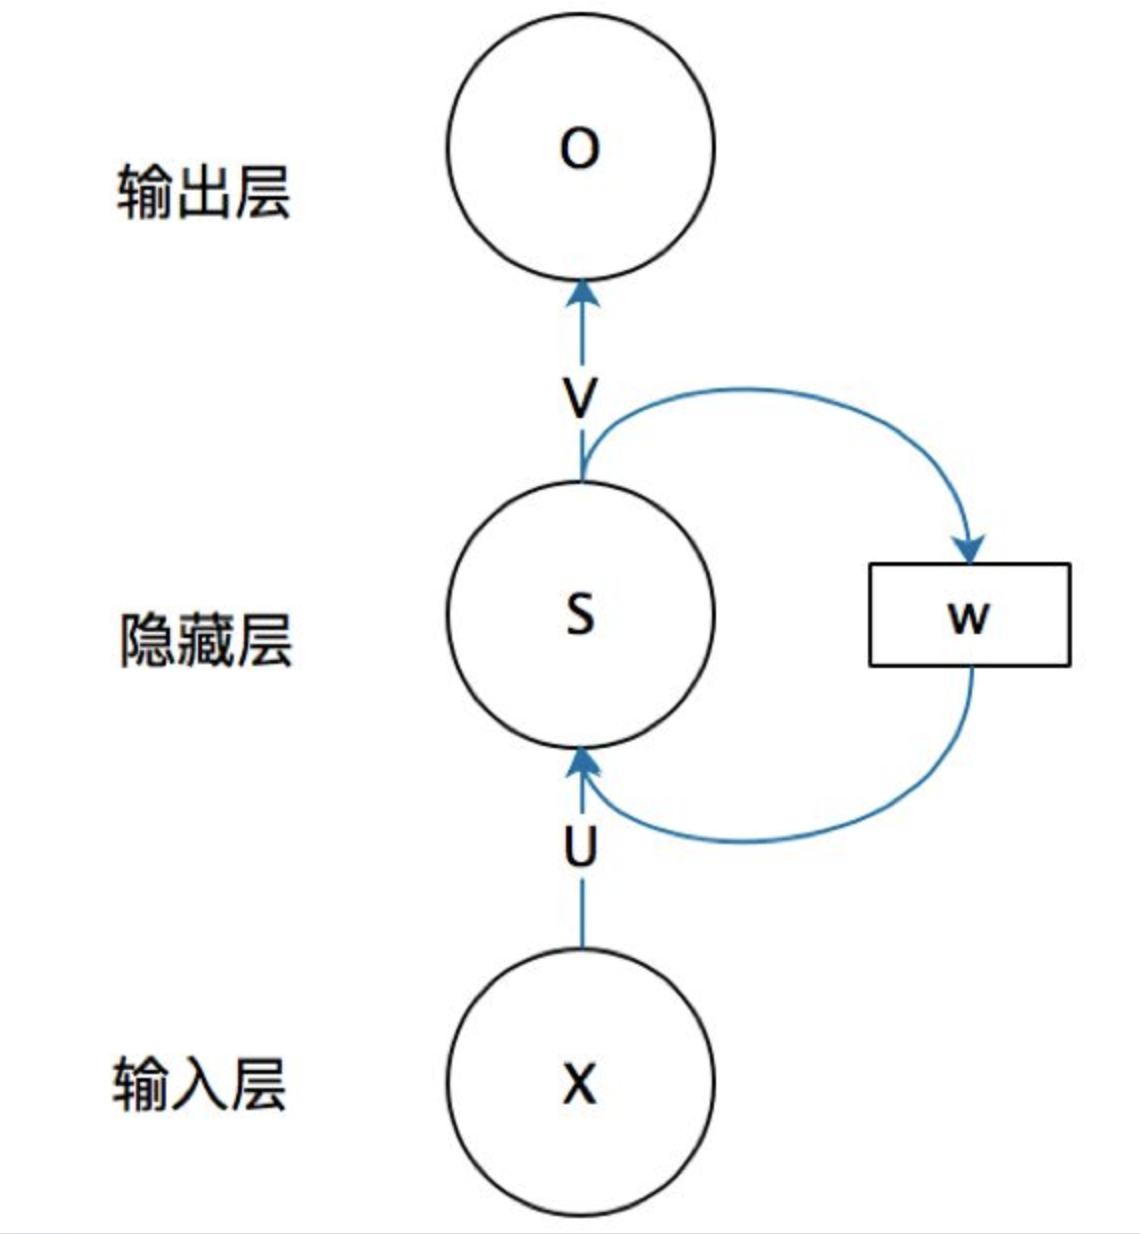
\includegraphics[width=.4\textwidth]{fig/RNN_Structure_Simple.png}
\end{figure}

我们现在这样来理解,如果把上面有W的那个带箭头的圈去掉,它就变成了最普通的全连接神经网络。x是一个向量,它表示输入层的值(这里面没有画出来表示神经元节点的圆圈);s是一个向量,它表示隐藏层的值(这里隐藏层面画了一个节点,你也可以想象这一层其实是多个节点,节点数与向量s的维度相同);

U是输入层到隐藏层的权重矩阵,o也是一个向量,它表示输出层的值;V是隐藏层到输出层的权重矩阵。

那么,现在我们来看看W是什么。\textbf{循环神经网络的隐藏层的值s不仅仅取决于当前这次的输入x,还取决于上一次隐藏层的值s}。权重矩阵 W就是隐藏层上一次的值作为这一次的输入的权重。

我们给出这个抽象图对应的具体图:
\begin{figure}[H]
    \centering
    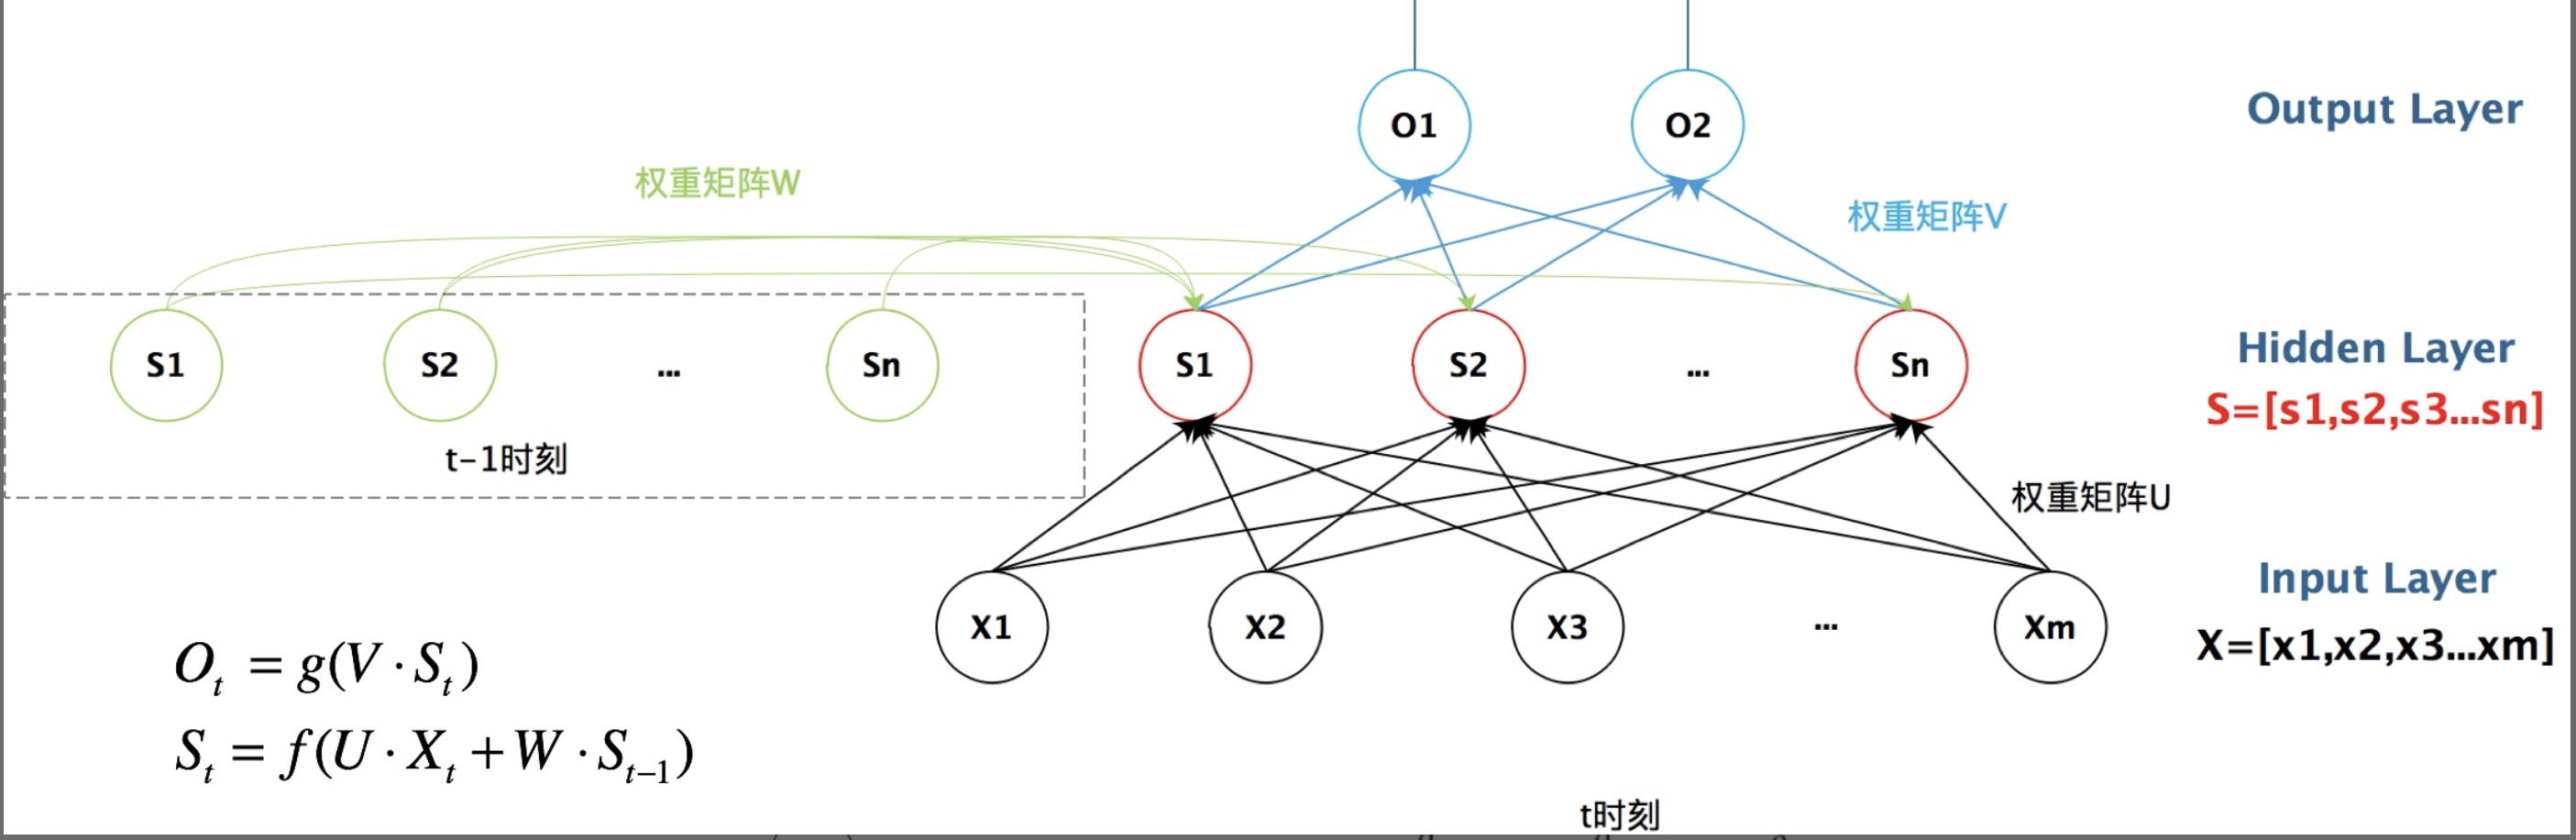
\includegraphics[width=1\textwidth]{fig/RNN_Structure_Detail.png}
\end{figure}

我们从上图就能够很清楚的看到,上一时刻的隐藏层是如何影响当前时刻的隐藏层的,注意:
$$
S_t = f(U\cdot X_t + W \cdot \mathbf{S_{t-1}})
$$

也就是说,$S_t$ 不仅收到输入向量$X_t$的影响,还收到上一时刻的$S_{t-1}$的影响。

如果我们把上面的图展开,循环神经网络也可以画成下面这个样子:
\begin{figure}[H]
    \centering
    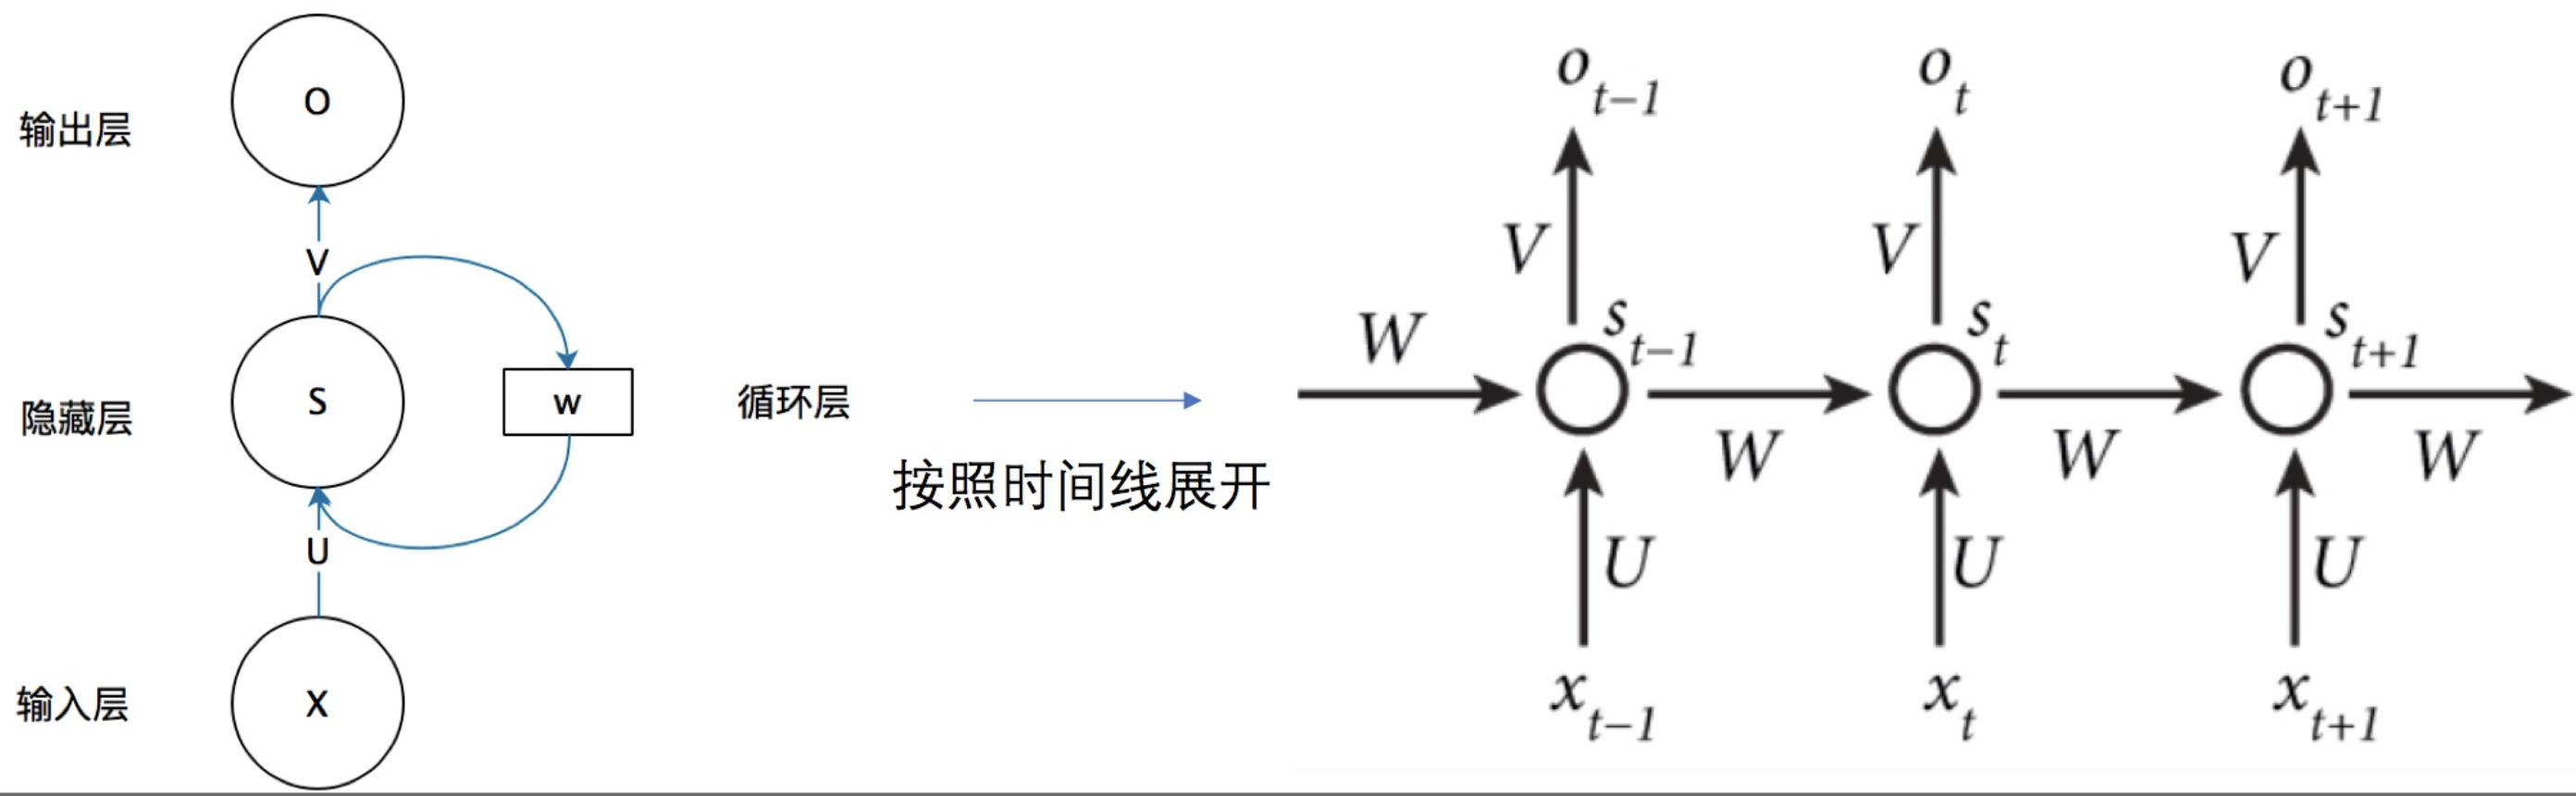
\includegraphics[width=1\textwidth]{fig/RNN_Structure_Expand_By_Time.png}
\end{figure}

现在看上去就比较清楚了,这个网络在$t$时刻接收到输入$x_t$ 之后,隐藏层的值是 $s_t$ ,输出值是$o_t$ 。关键一点是,$s_t$ 的值不仅仅取决于$x_t$,还取决于 $s_{t-1}$ 。我们可以用下面的公式来表示循环神经网络的计算方法:
\begin{align*}
S_t &= f(U\cdot X_t + W \cdot S_{t-1}) \\
O_t &= g(V \cdot S_t) \\
\end{align*}

\begin{framed}
从下面这张图,也可以很容易理解RNN的结构:
\begin{figure}[H]
    \centering
    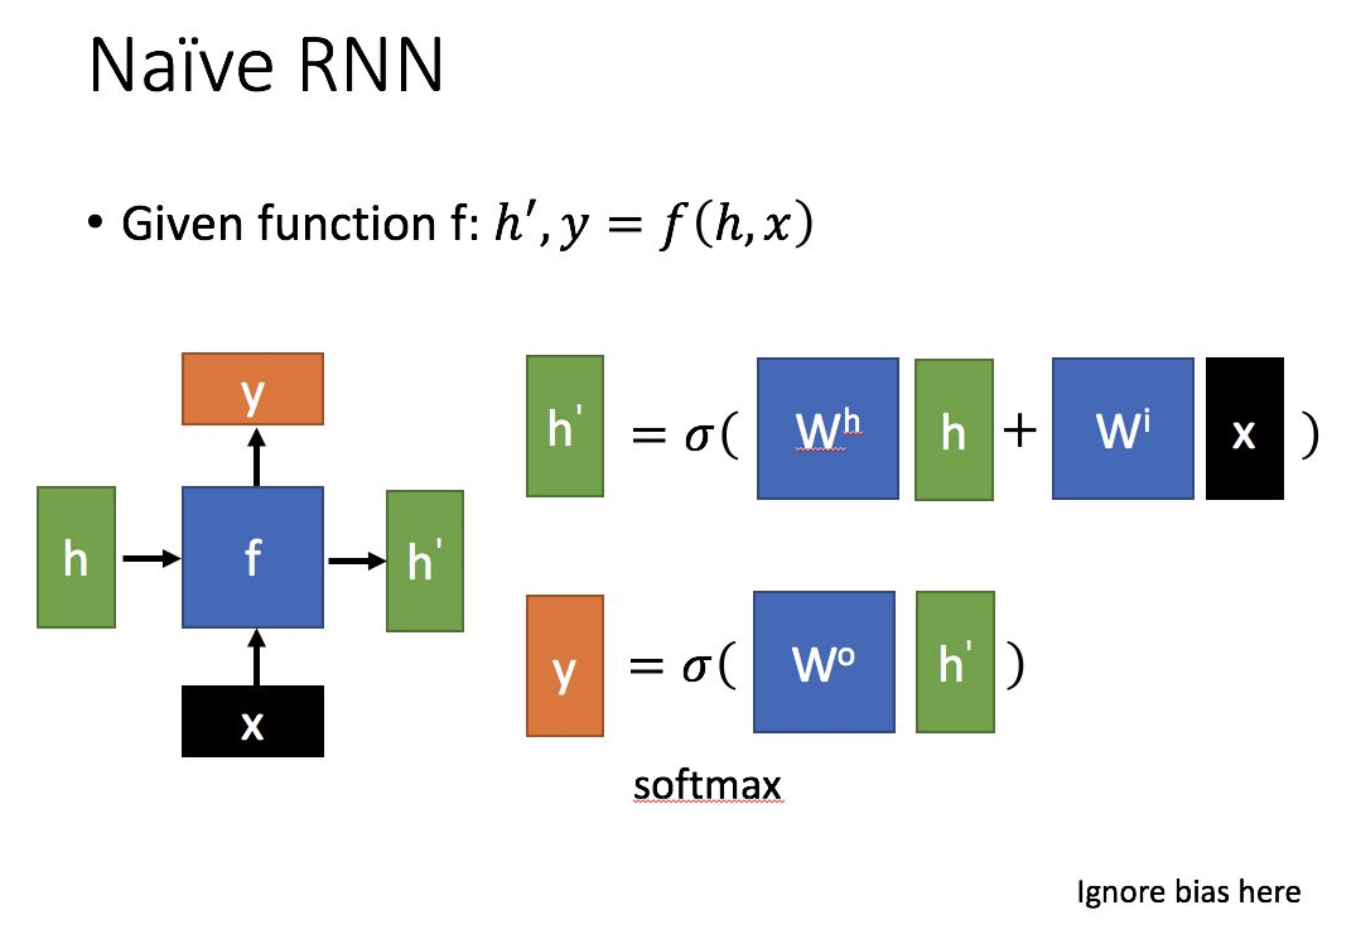
\includegraphics[width=.6\textwidth]{fig/RNN_Naive_Structure.png}
\end{figure}

$x_t$为当前状态下数据的输入; $h$表示接收到的上一个节点的输入。

$y$ 为当前节点状态下的输出,而 $h'$ 为传递到下一个节点的输出。

通过上图的公式可以看到,输出 $h'$ 与 $x$ 和 $h$ 的值都相关。而 $y$ 则常常使用 $h'$ 投入到一个线性层(主要是进行维度映射)然后使用softmax进行分类得到需要的数据。

对这里的$y$如何通过 $h'$ 计算得到往往看具体模型的使用方式。

通过序列形式的输入,我们能够得到如下形式的RNN。
\begin{figure}[H]
    \centering
    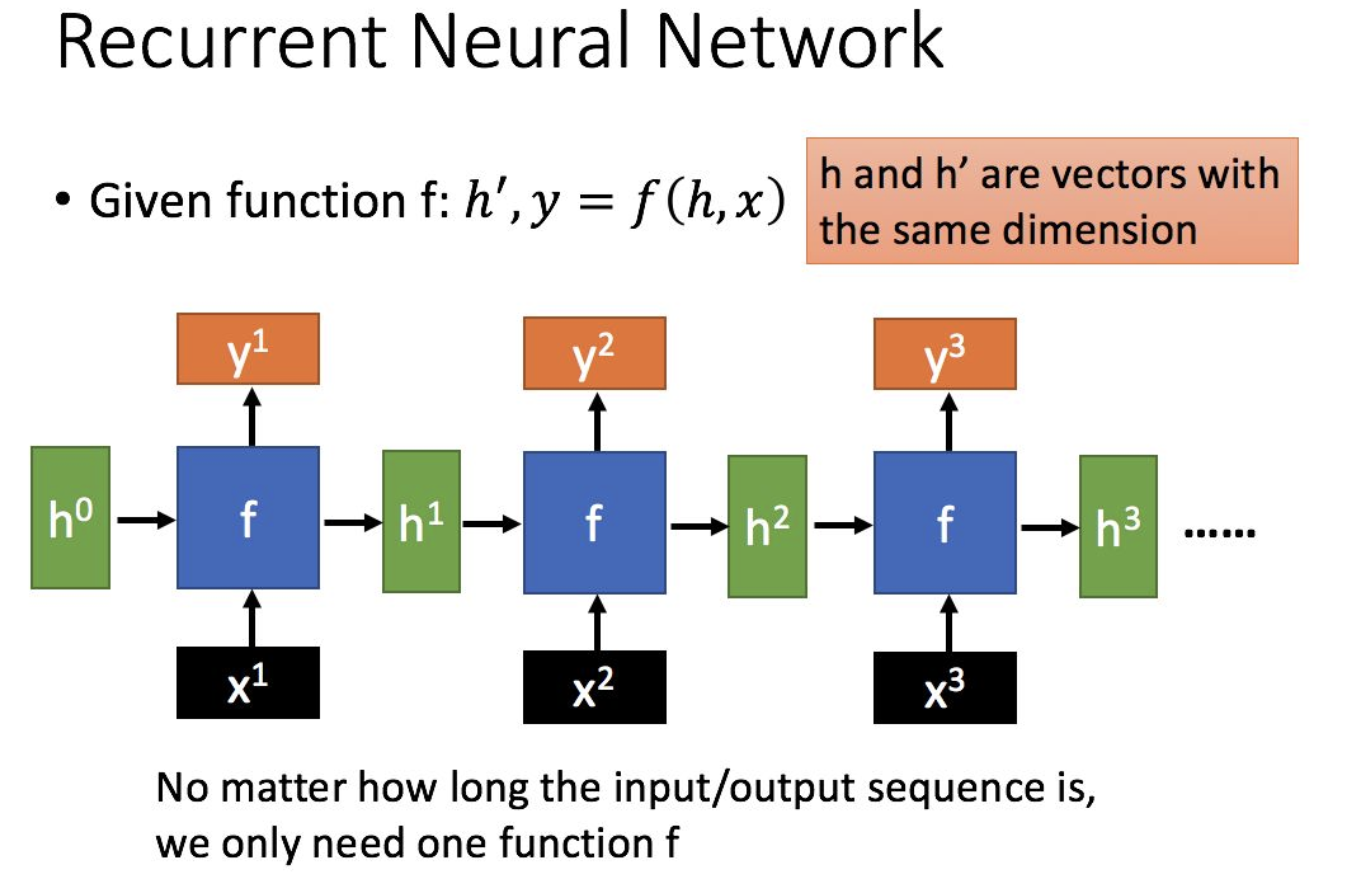
\includegraphics[width=.6\textwidth]{fig/RNN_Naive_Structure_Expand.png}
\end{figure}
\end{framed}

\subsection{RNN 深入理解\cite{Deep_Understand_RNN_And_LSTM}}
RNN的特征在于,\textbf{对于每个RNN神经元,其参数始终共享,即对于文本序列,任何一个输入都经过相同的处理,得到一个输出}。在传统的全连接神经网络的结构中,神经元之间互不影响,并没有直接联系,神经元与神经元之间相互独立。而在RNN结构中,隐藏层的神经元开始通过一个隐藏状态所相连,通常会被表示为 $h_t$ 。在理解RNN与全连接神经网络时,需要对两者的结构加以区分,通常,FCN会采用水平方式进行可视化理解,即每一层的神经元垂直排列,而不同层之间以水平方式排布。但在RNN的模型图中,隐藏层的不同神经元之间通常水平排列,而隐藏层的不同层之间以垂直方式排列,如图所示,在FCN网络中,各层水平布局,隐藏层各神经元相互独立,在RNN中,各层以垂直布局,而水平方向上布局着各神经元。\textbf{注意:RNN结构图只是为了使得结构直观易理解,而在水平方向上其实每个A都相同,对于每个时间步其都是采用同一个神经元进行前向传播}。
\begin{figure}[H]
    \centering
    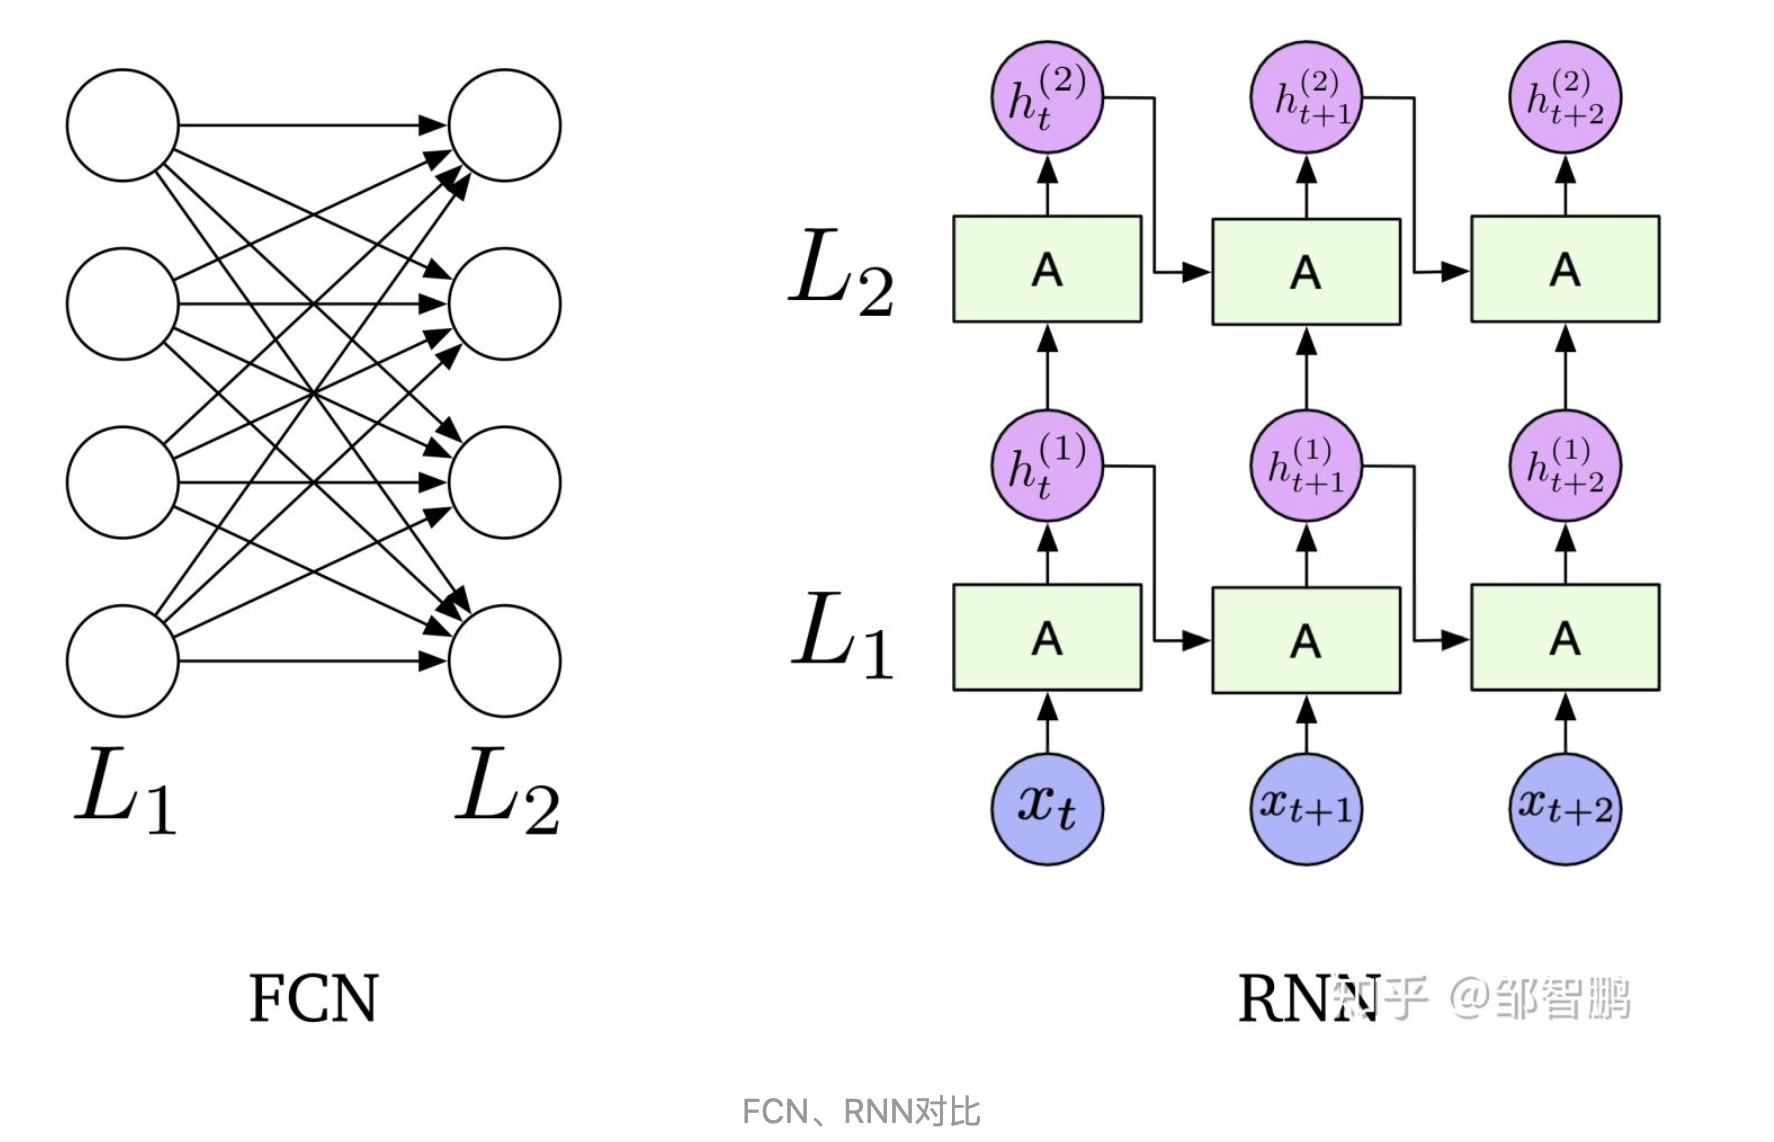
\includegraphics[width=.6\textwidth]{fig/RNN_Compare_FCN_RNN_Structure.png}
\end{figure}

\subsection{RNN的前向传播}
在RNN中,序列数据按照其时间顺序,依次输入到网络中,而时间顺序则表示时间步的概念。在RNN中,隐藏状态极为重要,隐藏状态是连接各隐藏层各神经元的中介值。如上图,在第一层中,在时间步 $t$ ,RNN隐藏层神经元得到隐藏状态$h_t^{(1)}$ ,在时间步$t+1$ ,则接受来自上一个时间步的隐藏层输出$h_t^{(1)}$,得到新的隐藏状态$h_{t+1}^{(1)}$ 。而从垂直方向上看,各层之间,也通过隐藏状态所连接,对于$L_1$ 到$L_2$ , $L_2$在水平的时间轴上,各神经元通过隐藏状态$h_t^{(2)}$连接,而层间还将接受前一层的$h_t^{(1)}$的值来作为$x_t$的值,从而获得到该层新的隐藏状态。因此,\textbf{RNN是一个在水平方向和垂直方向上,均可扩展的结构}(水平方向上只是人为添加的易于理解的状态,在工程实践中不存在水平方向的设置)。

根据RNN的定义,可以简单地给出RNN的前向传播过程:
$$
h_t = g(Wx_t + Vh_{t-1} + b)
$$

如上式,对于某一层, $W,V,b$均为模型需要学习的参数,通过上图RNN结构图的对应,则应为$L_1$层水平方向所有神经元的参数,\textbf{同一层的RNN单元参数相同,即参数共享}。若考虑多层RNN,则可将上式改为:
$$
h_t^{[i]} = g(W^{[i]}x_t^{[i-1]} + V^{[i-1]}h_{t-1}^{[i]} + b^{[i]})
$$

为了简化研究,下文统一对单层RNN进行讨论。值得注意的是,单层RNN前向传播可做如下变换:
$$
Wx_t + Vh_{t-1} = \begin{bmatrix}
W & V
\end{bmatrix} \times \begin{bmatrix}
x_t \\ h_{t-1}
\end{bmatrix}
$$

为此,我们不妨将参数进行统一表示:$W = [W;V]$,其中 $[\cdot ; \cdot ]$表示拼接操作,则前向传播变为:
$$
h_t = g(W[h_{t-1};x_t]^T + b)
$$

在获得隐藏状态后,若需要获得每一个时间步的输出,则需要进一步进行线性变换:
$$
o_t = Vh_t + b_o; \qquad y_t = g(o_t)
$$

其中$V,b$为参数,$g(\cdot)$ 为激活函数,如
$$
\text{softmax} = \frac{\exp(x_j)}{\sum_{i=1}^n\exp(x_i)}
$$

\subsection{RNN的反向传播}
为简化分析,选用RNN的最后时间步的隐藏状态(无输出层)直接作为输出层,即$\text{output} = h_t = g(W[h_{t-1};x_t]^T+b)$ ,若为分类问题,则 $g(\cdot)$ 通常为 softmax 。定义问题的损失函数为$J(\theta) = \text{Loss}(\text{output}, y|\theta)$,则在进行反向传播时,需要计算 $W,b$的梯度,可进行如下推导:
\begin{align*}
\Delta W &= \frac{\partial J(\theta)}{\partial W}  = \frac{\partial}{\partial W}\text{Loss}(\text{output}, y) \\
	&= \text{Loss}(\text{output}, y)' \frac{\partial g(W[h_{t-1};x]^T+b)}{\partial W} \\
	&= \text{Loss}(\text{output},y)'g(\cdot)'[h_{t-1};x_t]
\end{align*}

然而,在RNN的反向传播中,\textbf{不仅需要根据垂直方向进行梯度推导,同时需要根据水平方向,按照时间步进行梯度推导,即RNN中的BPTT(Back Propagation Through Time)反向传播}。从公式中也可以看出,在前向传播过程中 $h_t$ 是关于$W$和$h_{t-1}$的函数值,即$h_t = f\Big(W[h_{t-1};x_t]^T+b\Big)$,则 $h_t$ 可以进一步进行微分,于是将 $h_t$关于 $W$ 求偏导,以循着时间轴更新$t-1$时刻的 $W$:
$$
\frac{\partial h_t}{\partial [h_{t-1};x_t]}\frac{\partial [h_{t-1};x_t]}{\partial W} = f(\cdot)'W[h_{t-2};x_{t-1}] \Rightarrow \Delta W_{t-1} = \text{Loss}(\text{output},y)'g(\cdot)'f(\cdot)'W[h_{t-1};x_{t-1}]
$$

根据反向传播的规则,每个在当前时间步 $t$ 应向前追溯直到 $t_0$,计算梯度并更新参数,而在RNN中时间步中的 $W$ 参数被所有步共享,因此梯度是对同一个参数计算,为此可以将梯度作求和,一次性更新至 $W$ ,如图每个箭头表示一次梯度计算,则在$t_3$时刻计算梯度时,不仅需要直接计算当前时刻的梯度,还仍需根据时间轴,分别计算
$t_2,t_1$ 时刻的梯度。

\begin{figure}[H]
    \centering
    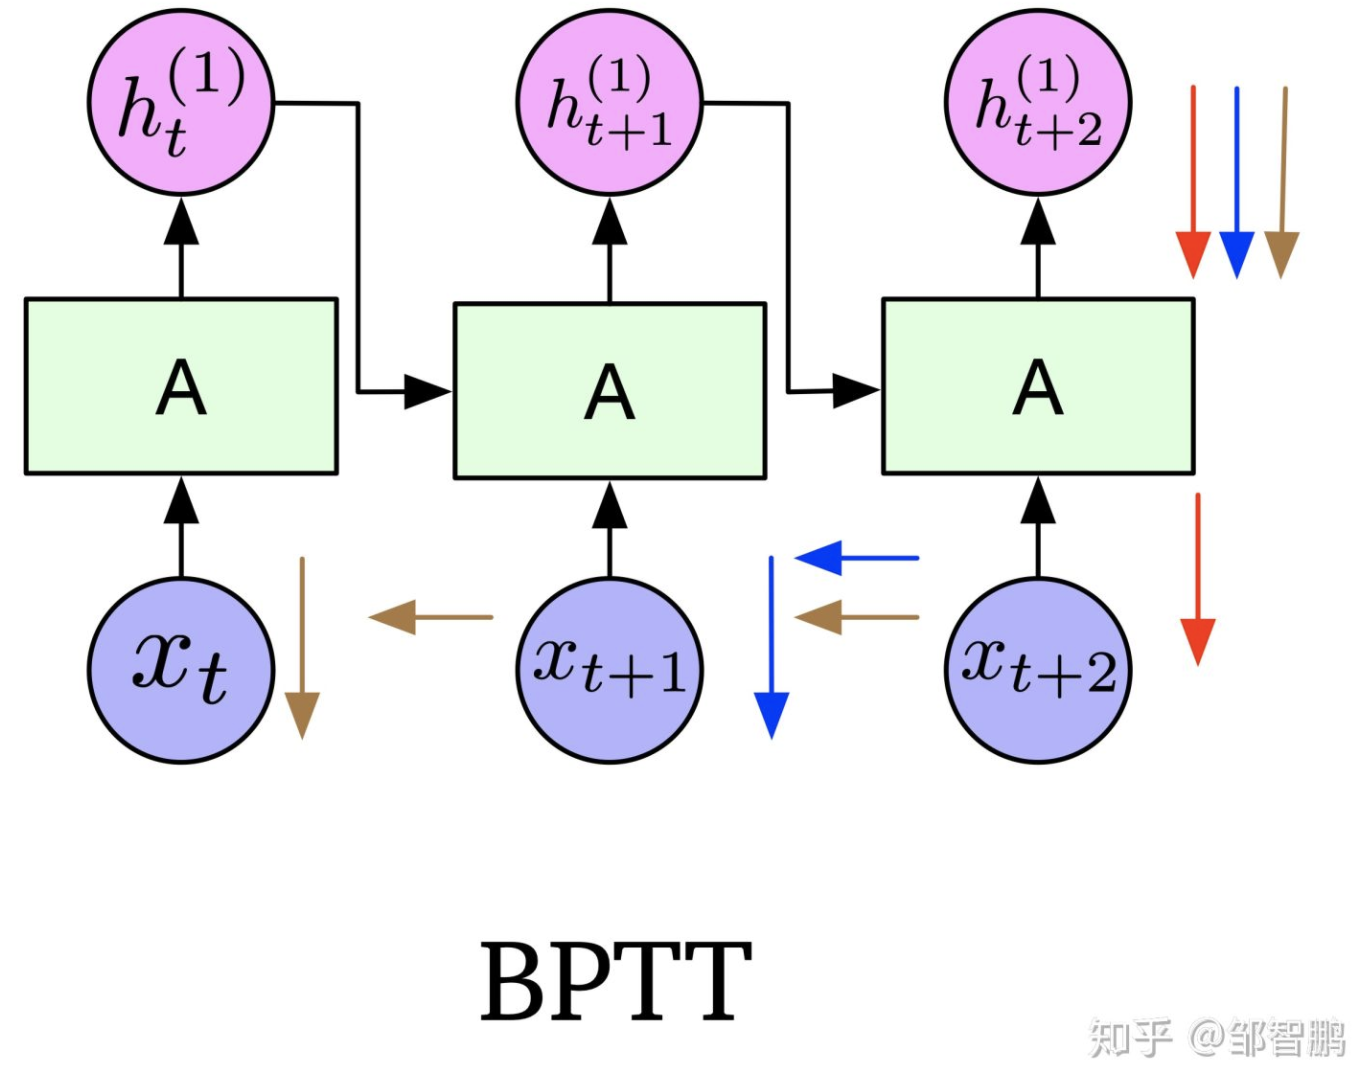
\includegraphics[width=.6\textwidth]{fig/RNN_BPTT_Process.png}
\end{figure}

注:本推导在假设RNN仅使用一个输出,即最后一个时间步的输出为最终输出,而RNN在每个时间步均有输出,若考虑多个输出,则损失函数不同,即损失为各时间步损失的总和,而在计算梯度时,需要对每个时间步输出均计算一个输出,即$\text{Loss} = \sum^tJ(\theta)$。

RNN 通常使用 tanh 函数,避免 sigmoid 导致的梯度消失的问题。

后略。

\subsection{RNN的问题}
来源:\url{https://zhuanlan.zhihu.com/p/115026734}

RNN的主要弱点是,善于进行短期记忆,不擅长进行长期记忆。由于激活函数(输出值取值范围[0,1])的存在,信息和残差在RNN神经元中传递时,会逐时间步损耗(简单来说就是绝对数值越来越小)。这个特点,削弱了RNN神经元保留距离当前时间步较远信息的能力,或者说,弱弱了RNN刻画长序列的能力。假设我们要从“贪污和浪费是极大的犯罪”抽取近义词,当模型从左到右、处理到”犯罪”的时候,“贪污”的语义已经被忘记,那么“犯罪-贪污”这对近义词就无法召回了。当然,实际发生的,是神经元“当前状态”,即语义向量里,所包含”贪污”越来越弱。看起来像是一个加权可以解决的问题。

\section{从 RNN 到 Seq2Seq 再到 Attention 机制\cite{Understand_RNN_Variants_Seq2Seq_Attention}}

\subsection{RNN的输出维度: N vs N}
下图是最经典的RNN结构。它的输入是x1, x2, .....xn,输出为y1, y2, ...yn,也就是说,\textbf{输入和输出序列必须要是等长的}。
\begin{figure}[H]
    \centering
    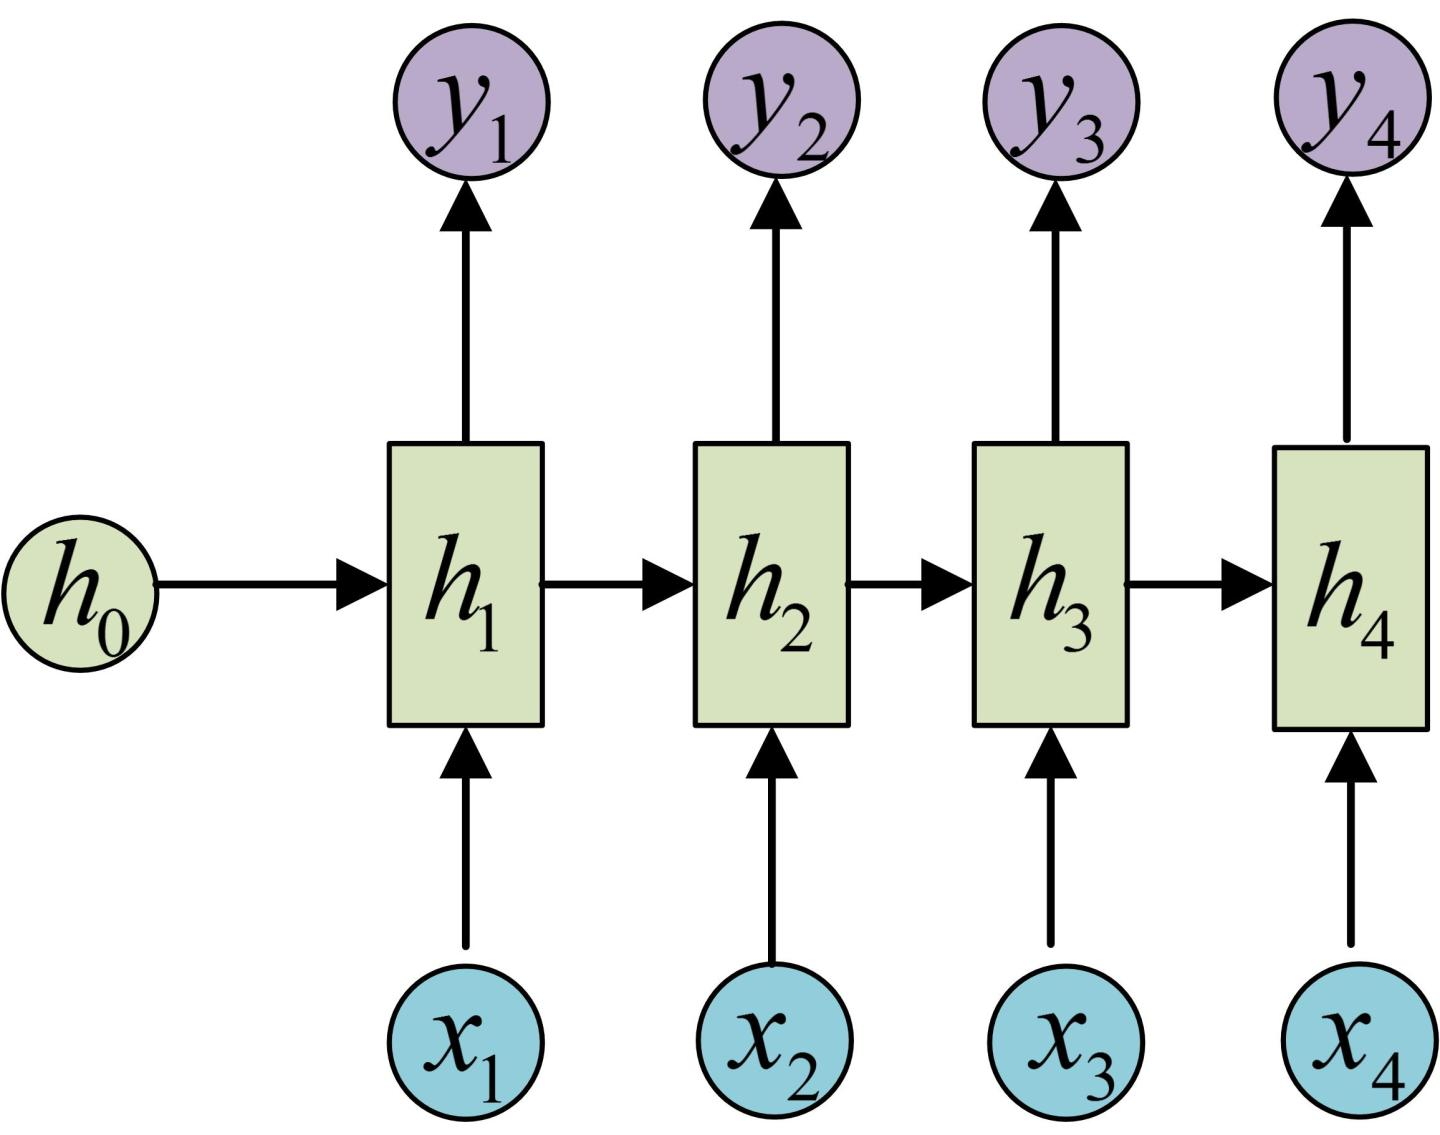
\includegraphics[width=.3\textwidth]{fig/RNN_Classic_Output_N_to_N.jpg}
\end{figure}

\subsection{RNN的输出维度:N vs 1}
有的时候,我们要处理的问题输入是一个序列,输出是一个单独的值而不是序列,应该怎样建模呢?实际上,我们只在最后一个$h$上进行输出变换就可以了:
\begin{figure}[H]
    \centering
    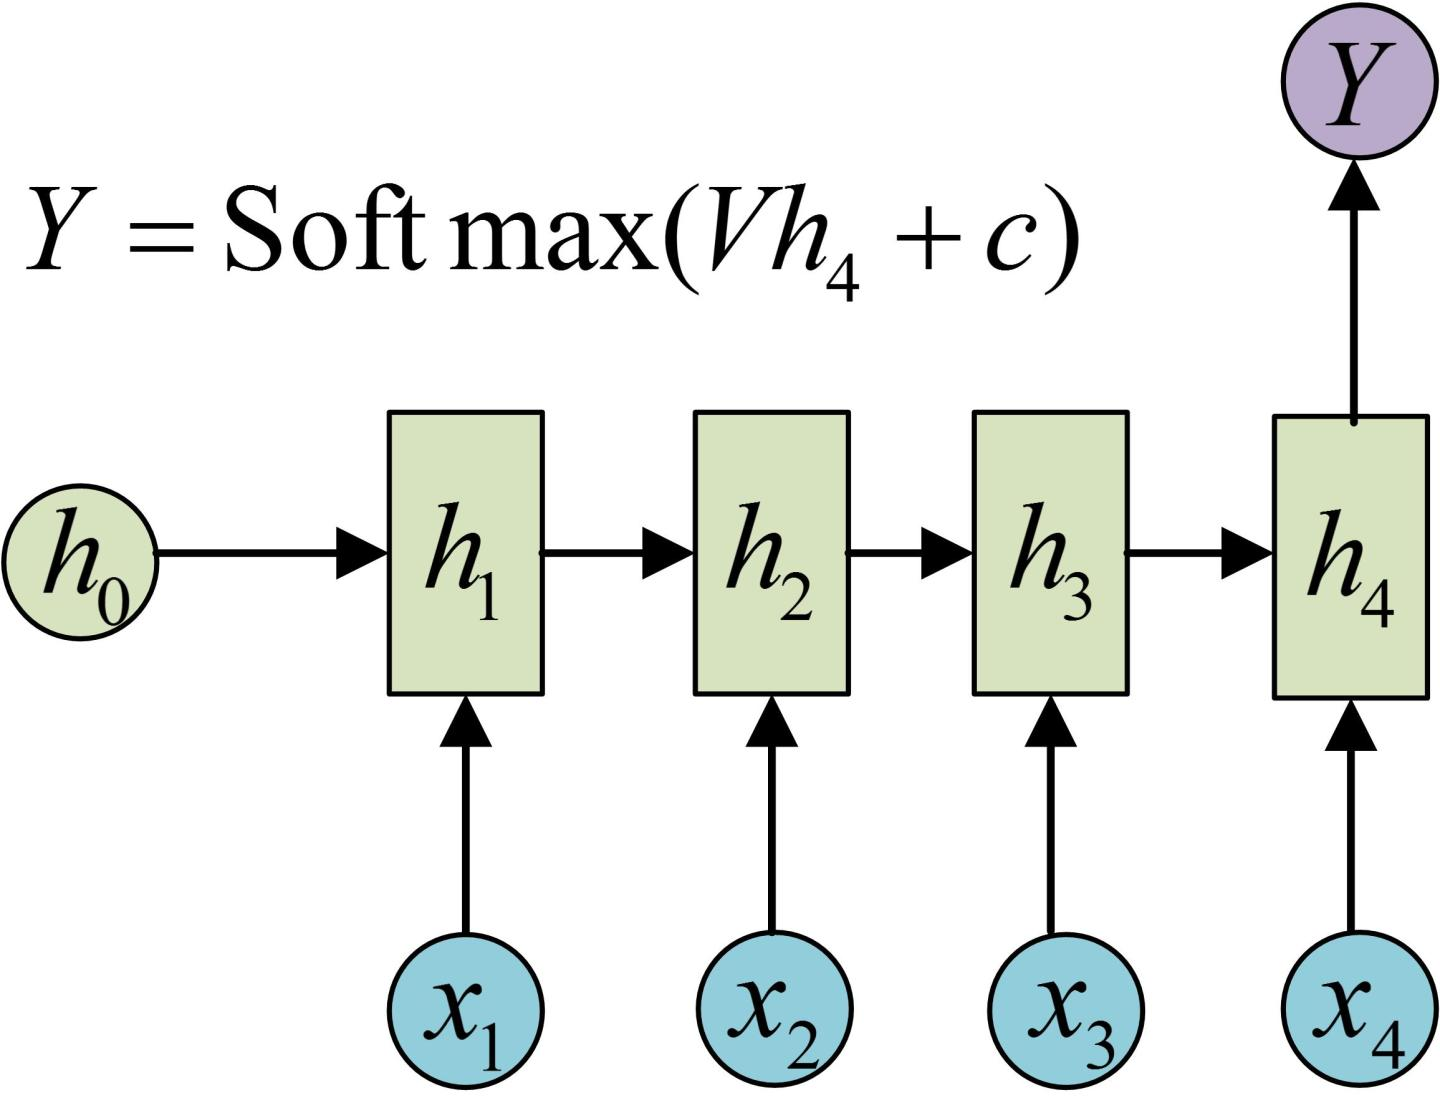
\includegraphics[width=.3\textwidth]{fig/RNN_Classic_Output_N_to_1.jpg}
\end{figure}

这种结构通常用来处理序列分类问题。如输入一段文字判别它所属的类别,输入一个句子判断其情感倾向,输入一段视频并判断它的类别等等。

\subsection{RNN的输出维度:1 vs N}
输入不是序列而输出为序列的情况怎么处理?我们可以只在序列开始进行输入计算:
\begin{figure}[H]
    \centering
    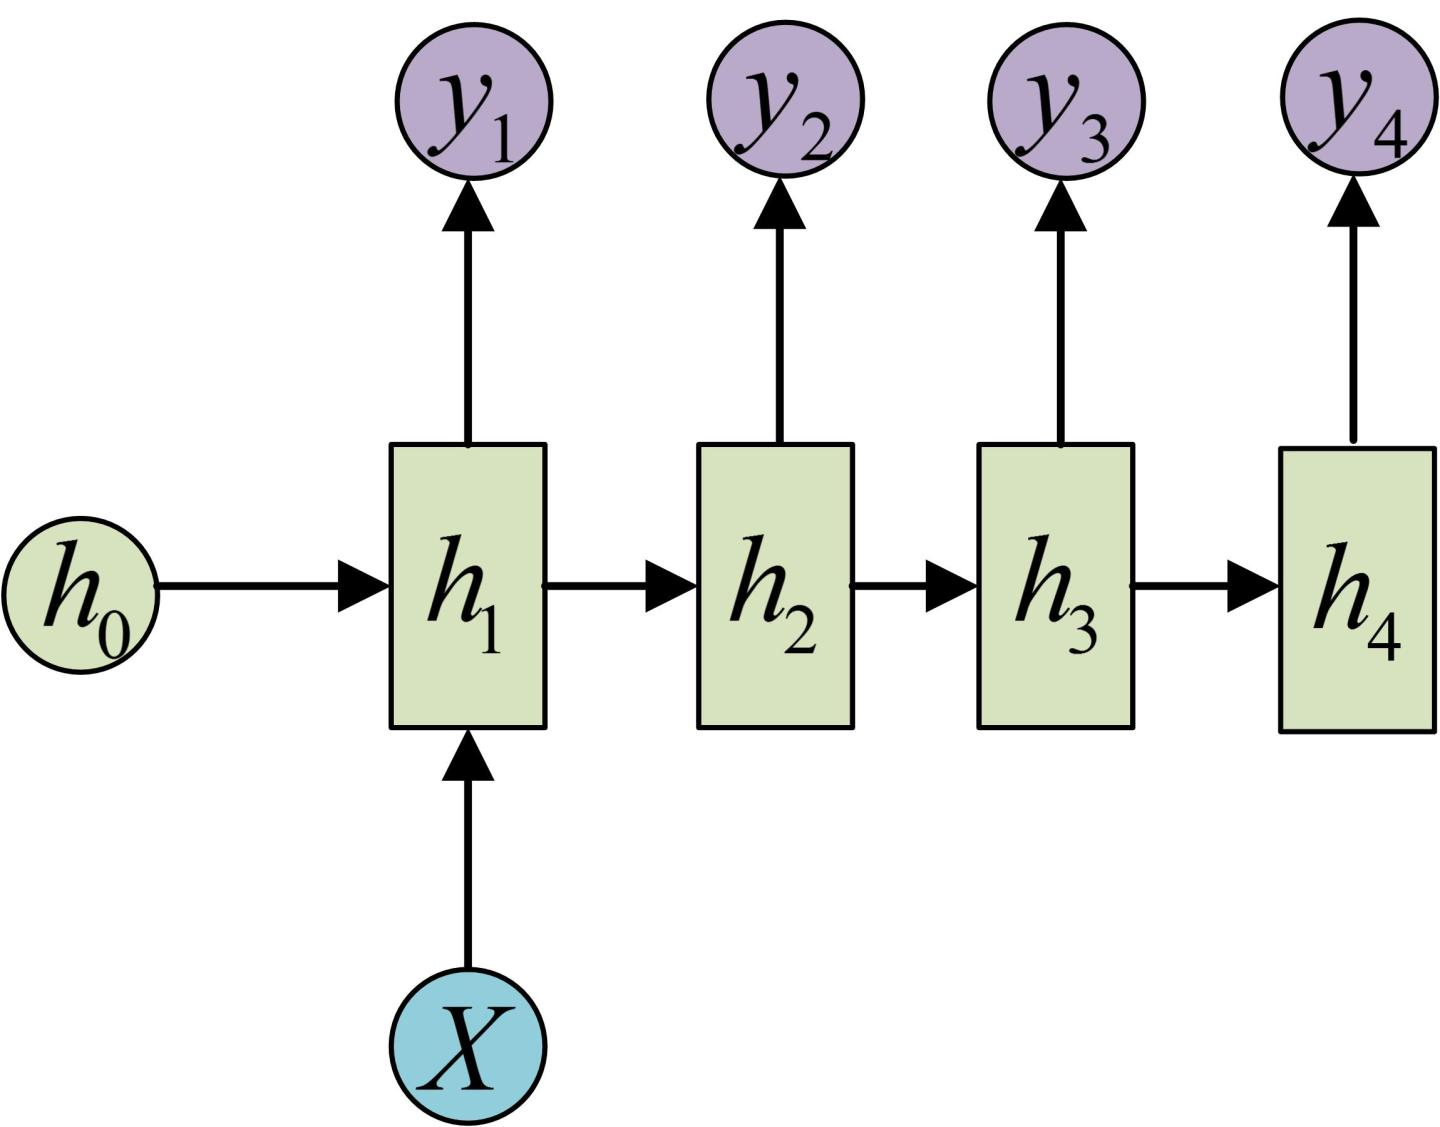
\includegraphics[width=.3\textwidth]{fig/RNN_Classic_Output_1_to_N.jpg}
\end{figure}

还有一种结构是把输入信息X作为每个阶段的输入:
\begin{figure}[H]
    \centering
    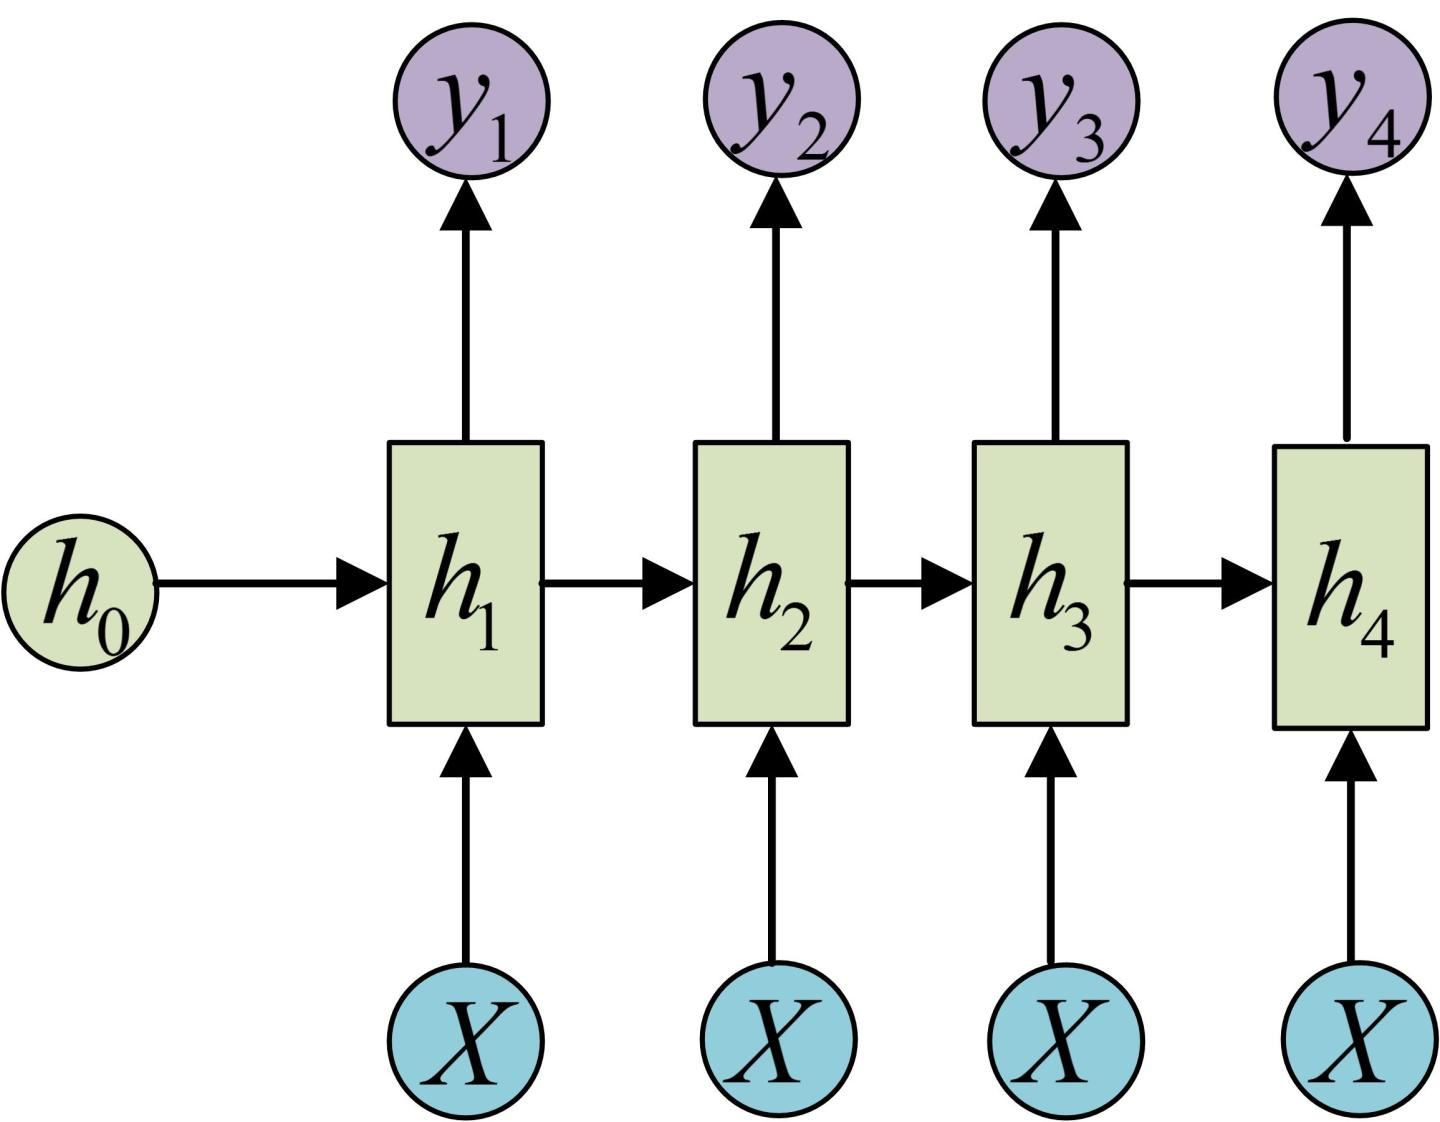
\includegraphics[width=.3\textwidth]{fig/RNN_Classic_Output_1_to_N_2.jpg}
\end{figure}

这种1 VS N的结构可以处理的问题有:从图像生成文字(image caption),此时输入的X就是图像的特征,而输出的y序列就是一段句子;从类别生成语音或音乐等。

\subsection{从 RNN 到 Seq2Seq}
下面我们来介绍RNN最重要的一个变种:N vs M。这种结构又叫Encoder-Decoder模型,也可以称之为Seq2Seq模型。

原始的N vs N RNN要求序列等长,然而我们遇到的大部分问题序列都是不等长的,如机器翻译中,源语言和目标语言的句子往往并没有相同的长度。\textbf{为此,Encoder-Decoder结构先将输入数据编码成一个上下文向量$c$}:
\begin{figure}[H]
    \centering
    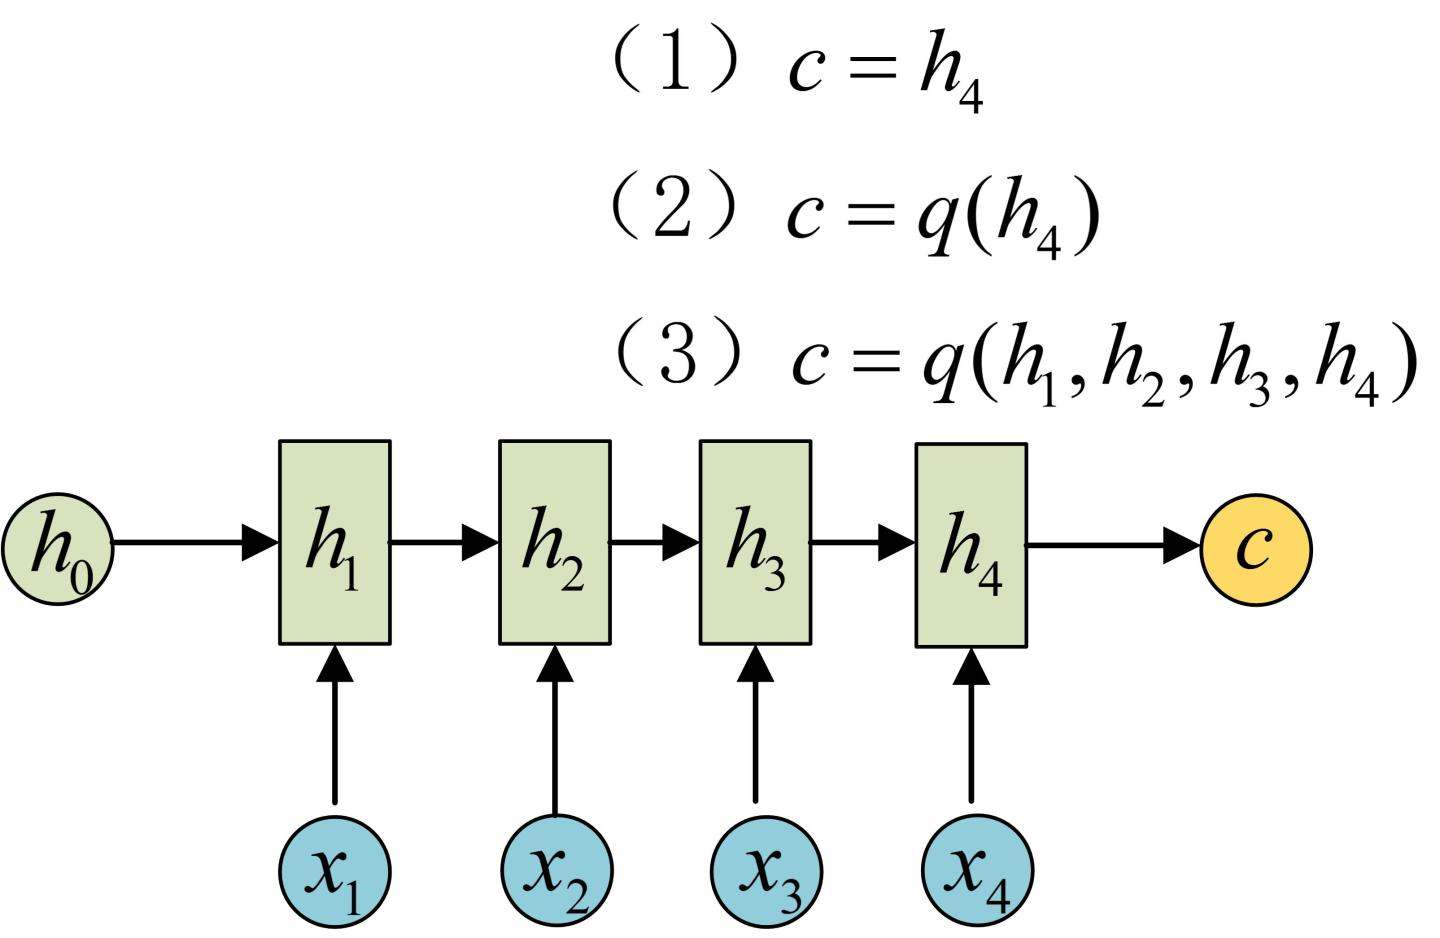
\includegraphics[width=.5\textwidth]{fig/RNN_Classic_Output_N_to_M_c.jpg}
\end{figure}

得到$c$有多种方式,最简单的方法就是把Encoder的最后一个隐状态赋值给$c$,还可以对最后的隐状态做一个变换得到$c$,也可以对所有的隐状态做变换。

\textbf{拿到c之后,就用另一个RNN网络对其进行解码},这部分RNN网络被称为Decoder。具体做法就是将$c$当做之前的初始状态$h_0$输入到Decoder中:
\begin{figure}[H]
    \centering
    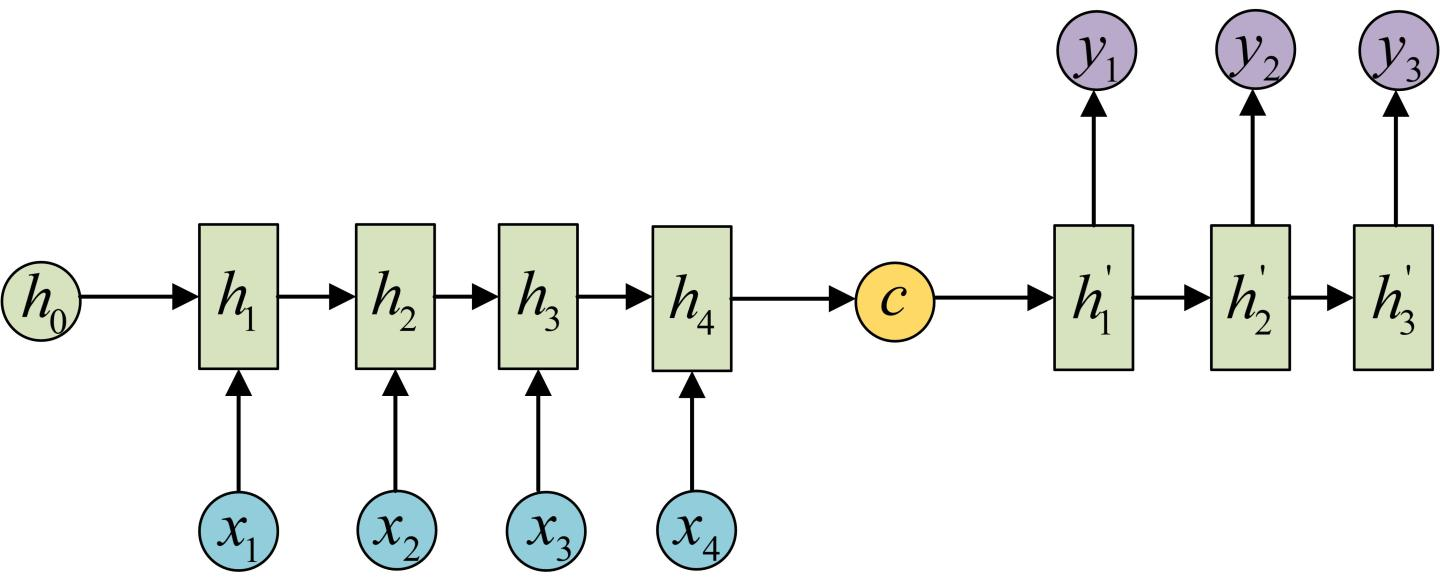
\includegraphics[width=.5\textwidth]{fig/RNN_Classic_Output_Encoder_Decoder.jpg}
\end{figure}

还有一种做法是将$c$当做每一步的输入:
\begin{figure}[H]
    \centering
    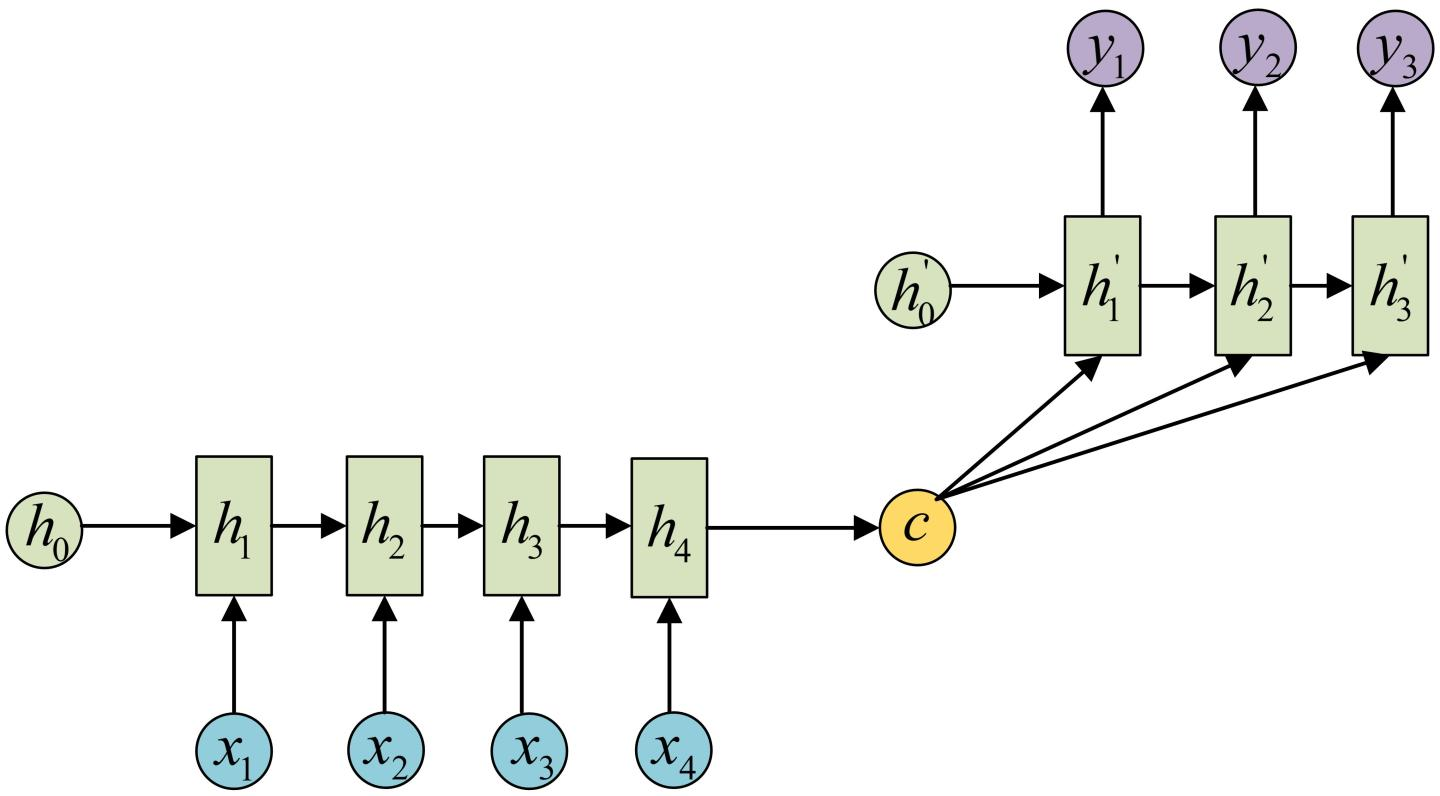
\includegraphics[width=.5\textwidth]{fig/RNN_Classic_Output_Encoder_Decoder_2.jpg}
\end{figure}

由于这种Encoder-Decoder结构不限制输入和输出的序列长度,因此应用的范围非常广泛,比如:
\begin{itemize}
\setlength{\itemsep}{0pt}
\setlength{\parsep}{0pt}
\setlength{\parskip}{0pt}
    \item 机器翻译。Encoder-Decoder的最经典应用,事实上这一结构就是在机器翻译领域最先提出的;
    \item 文本摘要。输入是一段文本序列,输出是这段文本序列的摘要序列;
    \item 阅读理解。将输入的文章和问题分别编码,再对其进行解码得到问题的答案;
    \item 语音识别。输入是语音信号序列,输出是文字序列;
    \item ……
\end{itemize}

\subsection{从 Seq2Seq 到 Attention 机制}
在Encoder-Decoder结构中,Encoder把所有的输入序列都编码成一个统一的语义特征c再解码,因此, \textbf{$c$中必须包含原始序列中的所有信息,它的长度就成了限制模型性能的瓶颈}。如机器翻译问题,当要翻译的句子较长时,一个$c$可能存不下那么多信息,就会造成翻译精度的下降。

Attention机制通过在每个时间输入不同的$c$来解决这个问题,下图是带有Attention机制的Decoder:
\begin{figure}[H]
    \centering
    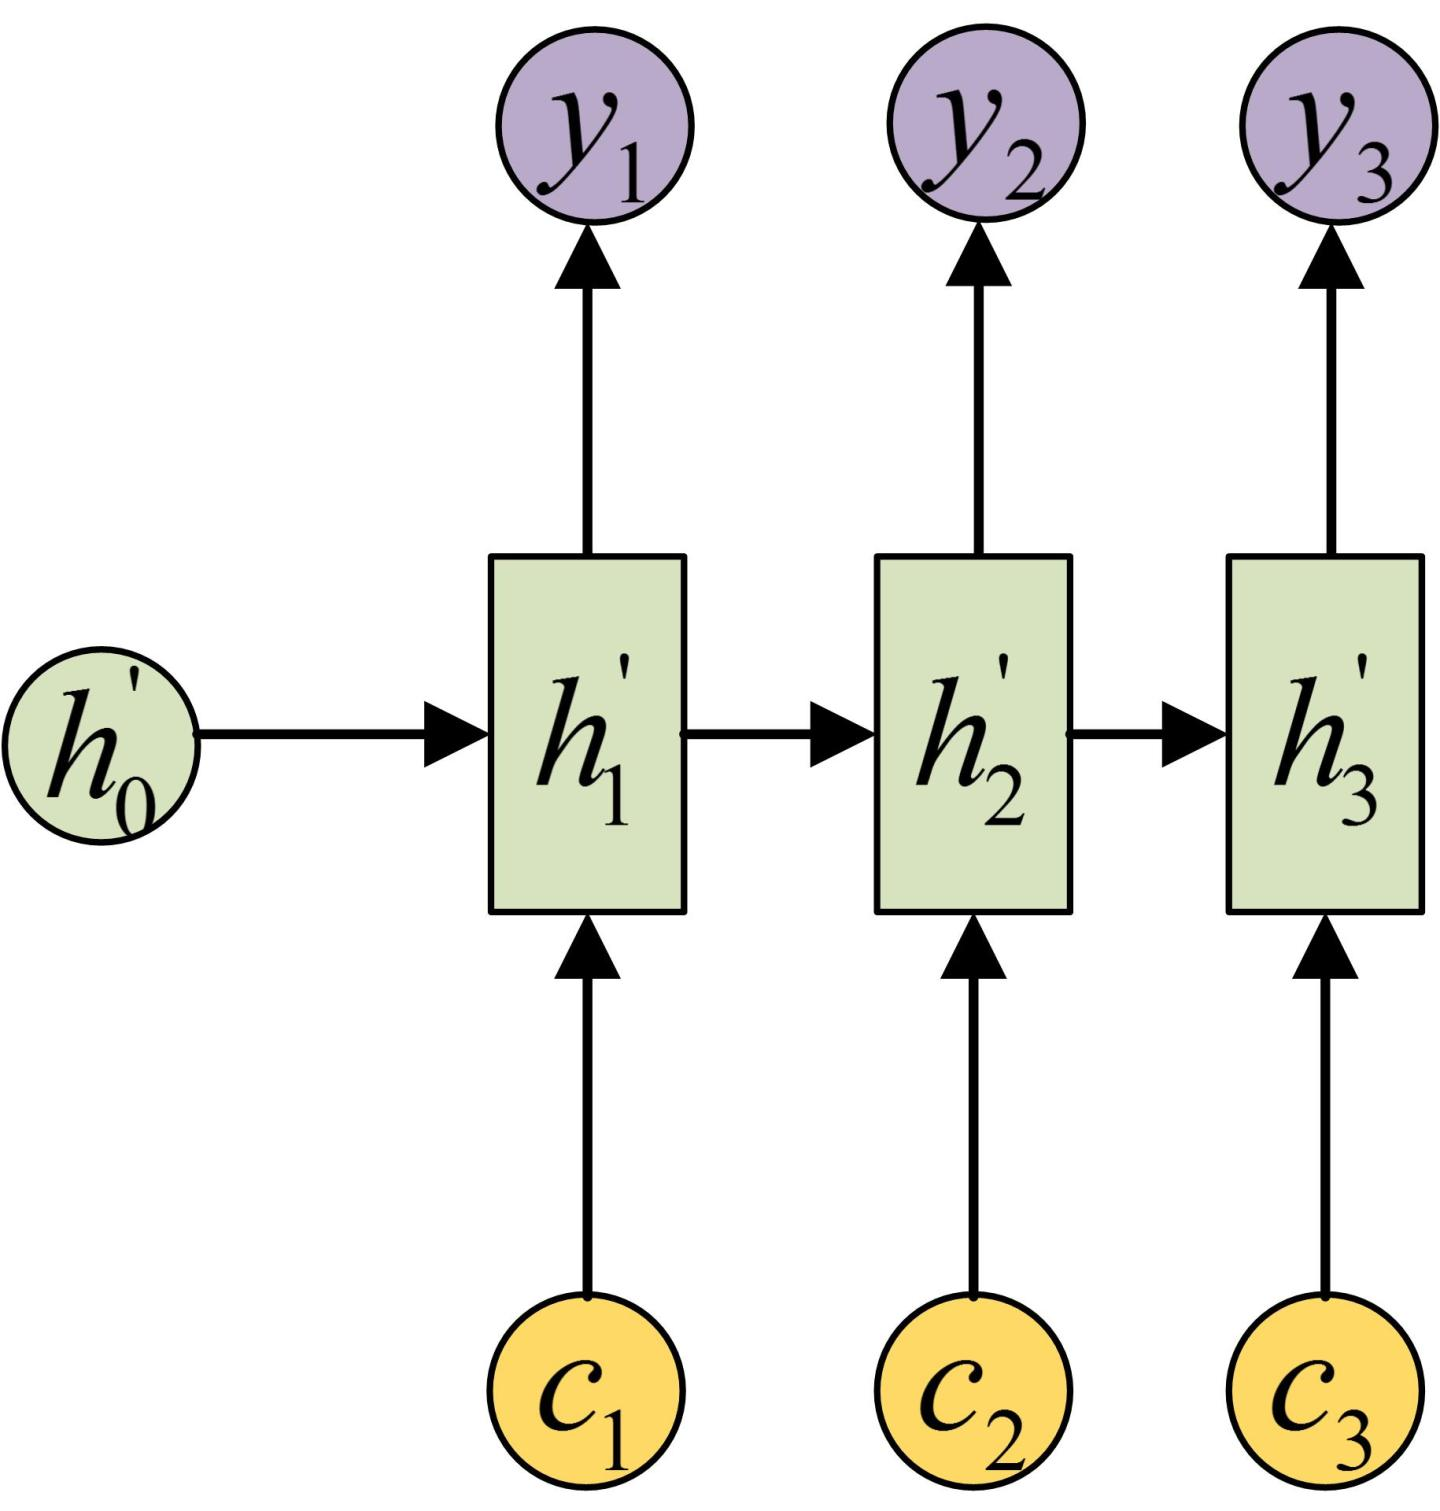
\includegraphics[width=.5\textwidth]{fig/Attention_Decoder_Different_C.jpg}
\end{figure}

\textbf{每一个$c$会自动去选取与当前所要输出的$y$最合适的上下文信息。具体来说,我们用 $a_{ij}$ 衡量Encoder中第$j$阶段的$h_j$和解码时第$i$阶段的相关性,最终Decoder中第$i$阶段的输入的上下文信息 $c_i$ 就来自于所有$h_j$对 $a_{ij}$ 的}\textcolor{red}{加权和}。

以机器翻译为例(将中文翻译成英文),输入的序列是“我爱中国”,因此,Encoder中的$h_1$、$h_2$、$h_3$、$h_4$就可以分别看做是“我”、“爱”、“中”、“国”所代表的信息。在翻译成英语时,第一个上下文$c_1$应该和“我”这个字最相关,因此对应的 $a_{11}$ 就比较大,而相应的 $a_{12}$ 、$a_{13}$、$a_{14}$就比较小。$c_2$ 应该和“爱”最相关,因此对应的$a_{22}$ 就比较大。最后的$c_3$和$h_3$、$h_4$最相关,因此$a_{33}$、 $a_{34}$ 的值就比较大。
\begin{figure}[H]
    \centering
    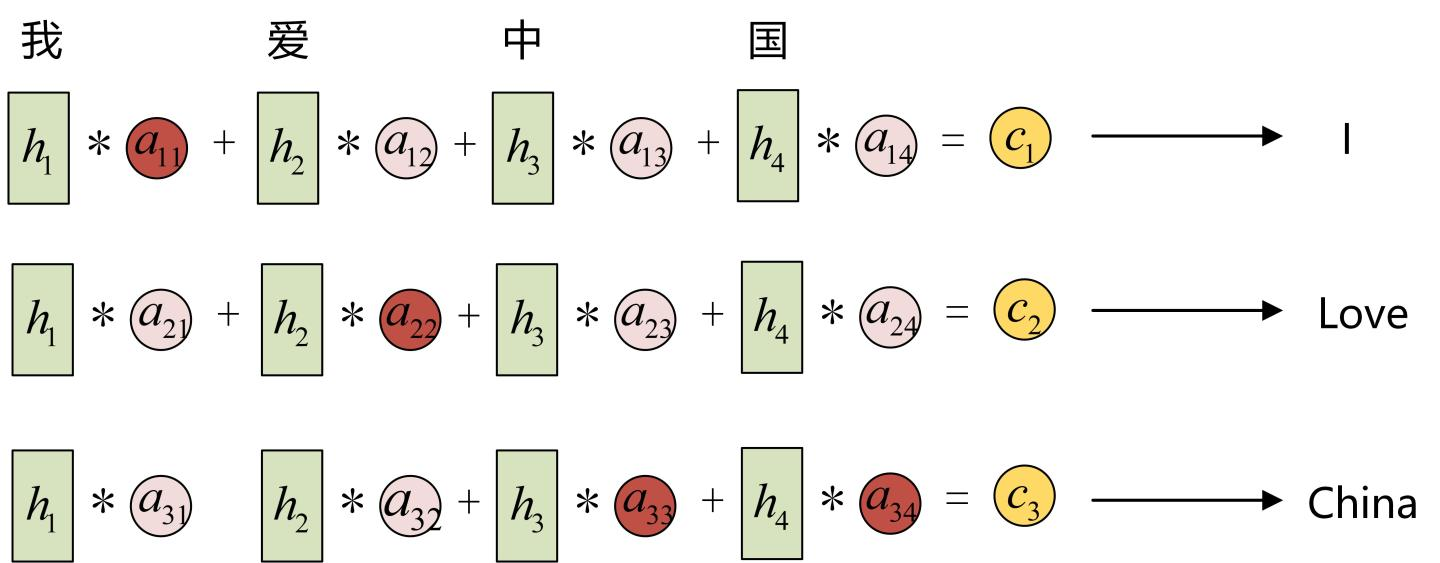
\includegraphics[width=.8\textwidth]{fig/Attention_Example.jpg}
\end{figure}

至此,关于Attention模型,我们就只剩最后一个问题了,那就是:这些权重 $a_{ij}$ 是怎么来的?

事实上,$a_{ij}$ 同样是从模型中学出的,它实际和Decoder的第$i-1$阶段的隐状态、Encoder第$j$个阶段的隐状态有关。

同样还是拿上面的机器翻译举例,$a_{1j}$ 的计算(此时箭头就表示对$h'$和 $h_j$ 同时做变换):
\begin{figure}[H]
    \centering
    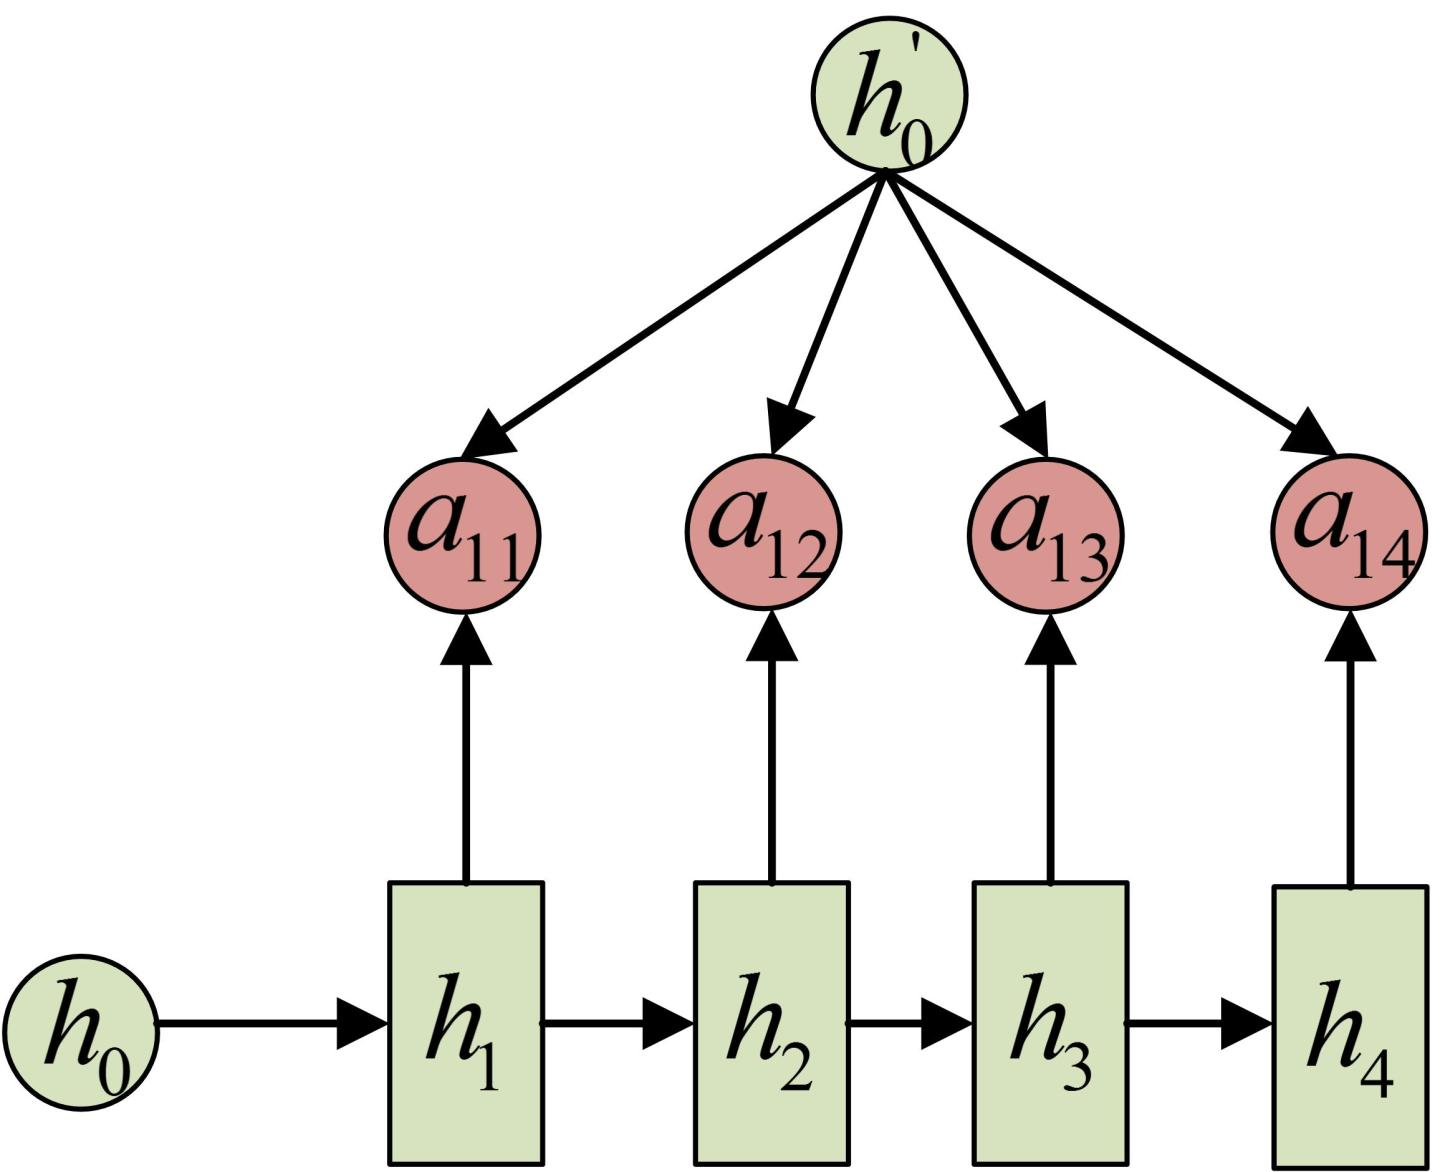
\includegraphics[width=.4\textwidth]{fig/Attention_Compute_A_1.jpg}
\end{figure}

$a_{2j}$ 的计算:
\begin{figure}[H]
    \centering
    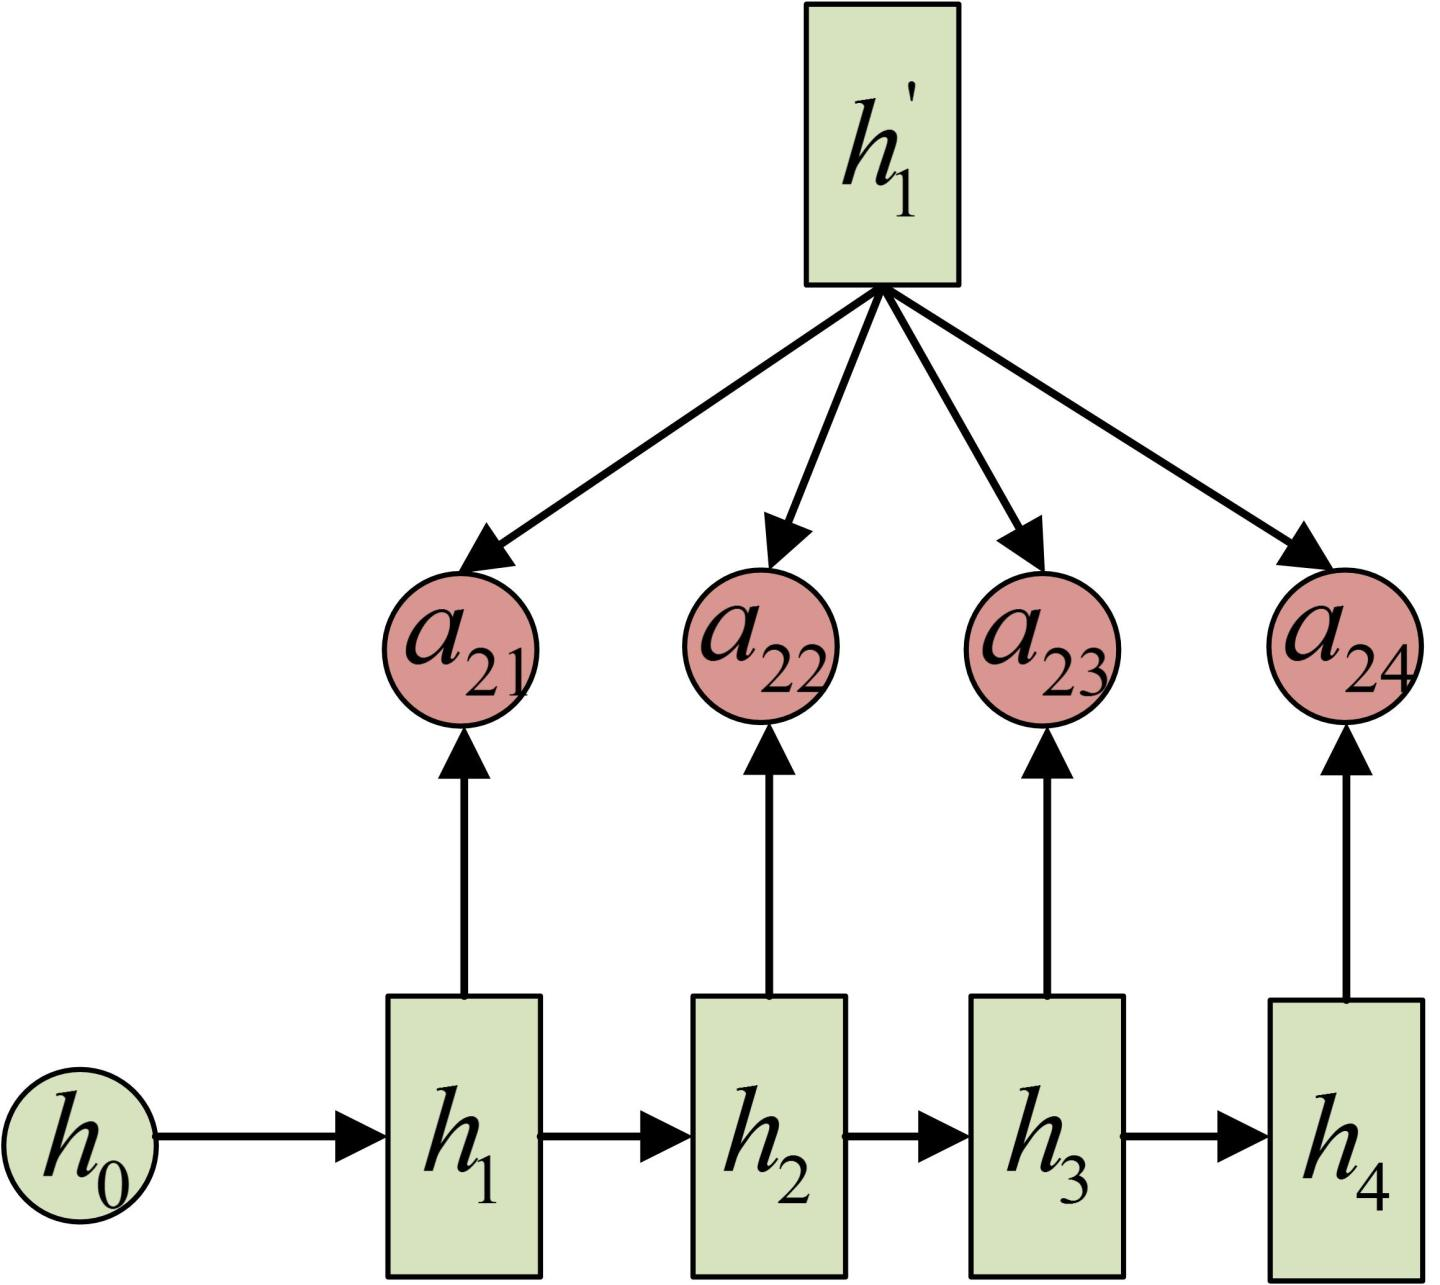
\includegraphics[width=.4\textwidth]{fig/Attention_Compute_A_2.jpg}
\end{figure}

$a_{3j}$ 的计算:
\begin{figure}[H]
    \centering
    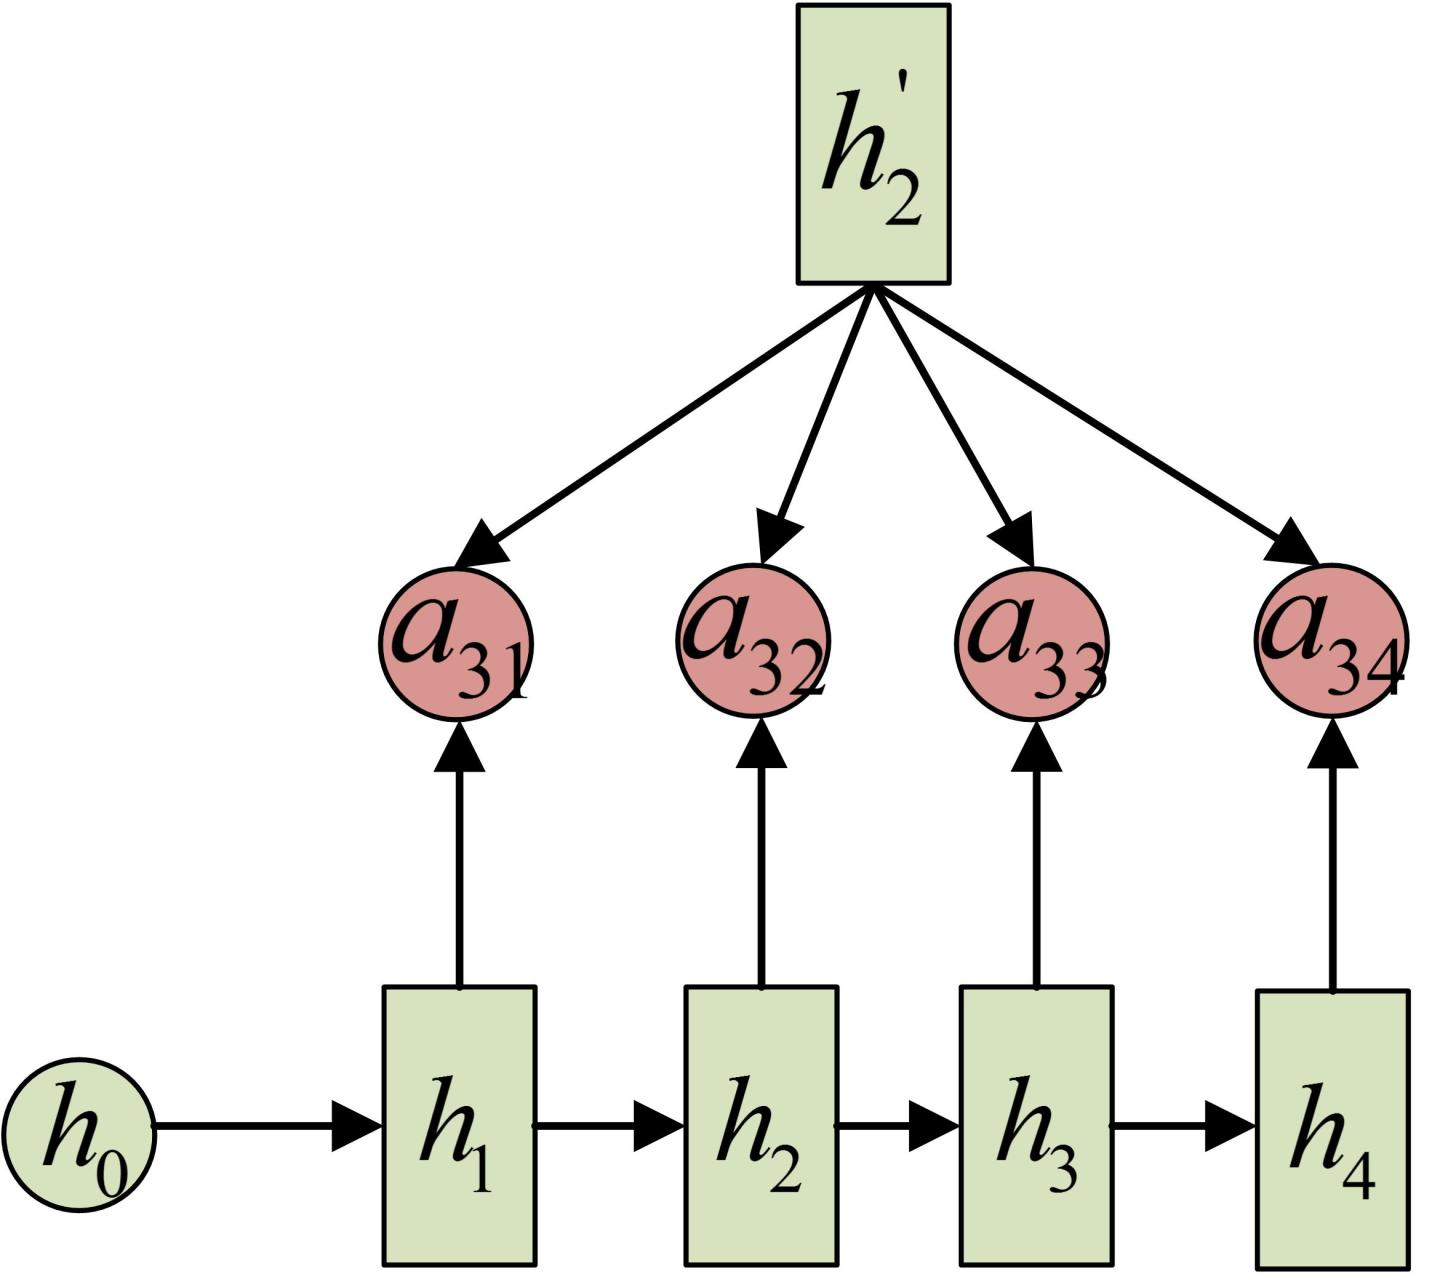
\includegraphics[width=.4\textwidth]{fig/Attention_Compute_A_3.jpg}
\end{figure}

以上就是带有Attention的Encoder-Decoder模型计算的全过程。



\section{ LSTM\cite{Everyone_Can_Understand_LSTM}}
\subsection{什么是LSTM}
长短期记忆(Long short-term memory, LSTM)是一种特殊的RNN,主要是为了解决长序列训练过程中的梯度消失和梯度爆炸问题。简单来说,就是相比普通的RNN,LSTM能够在更长的序列中有更好的表现。

LSTM结构(图右)和普通RNN的主要输入输出区别如下所示。
\begin{figure}[H]
    \centering
    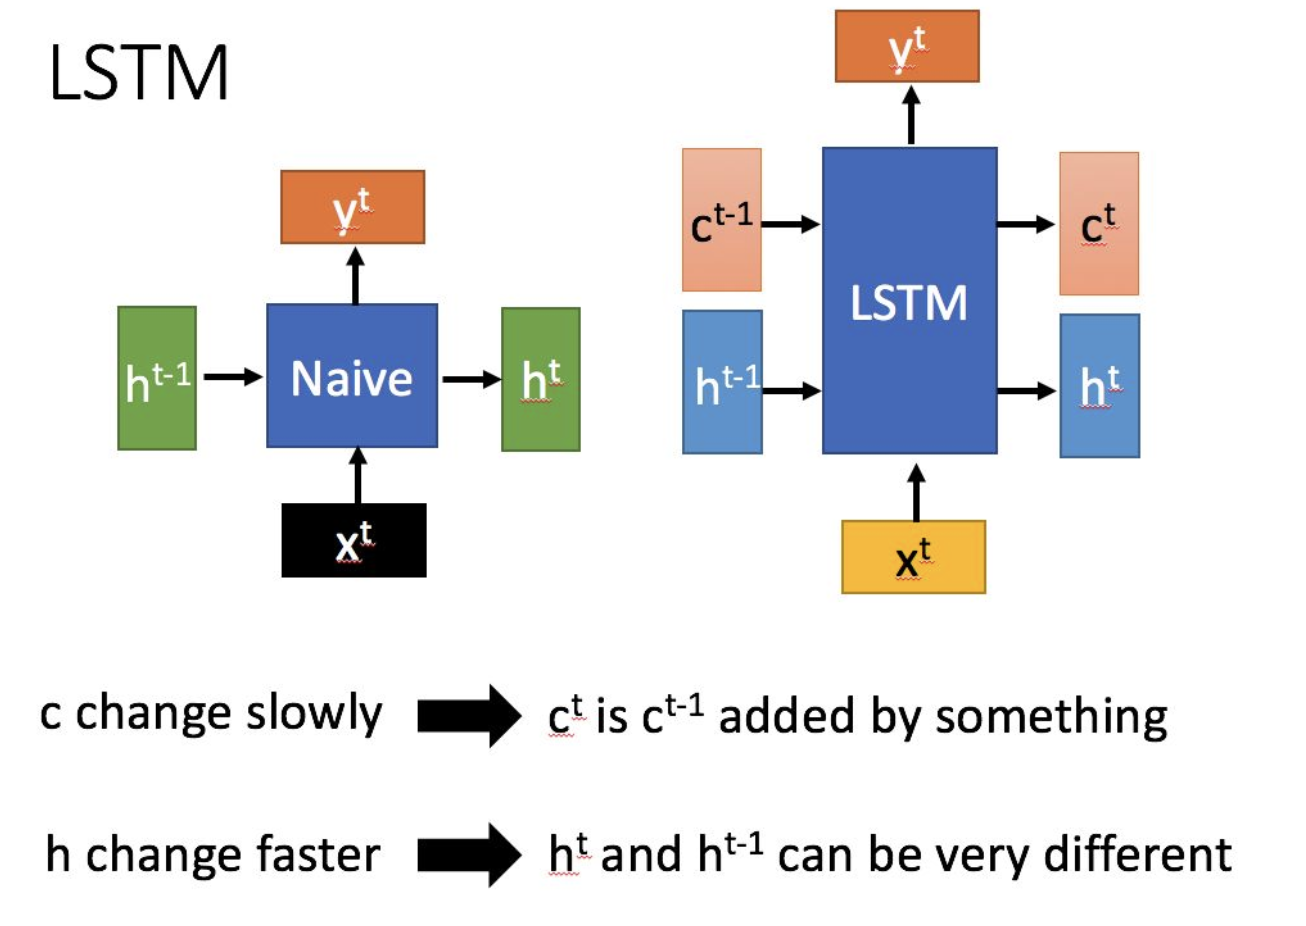
\includegraphics[width=.6\textwidth]{fig/LSTM_Compare_RNN_LSTM.png}
\end{figure}

\textbf{相比RNN只有一个传递状态$h^t$,LSTM有两个传输状态,一个 $c^t$ (cell state),和一个 $h^t$ (hidden state)。(Tips:RNN中的 $h^t$ 对于LSTM中的$c^t$ )}

其中对于传递下去的 $c^t$改变得很慢,通常输出的$c^t$ 是上一个状态传过来的 $c^{t-1}$ 加上一些数值;而$h^t$则在不同节点下往往会有很大的区别。

\subsection{深入LSTM结构}
下面具体对LSTM的内部结构来进行剖析。

首先使用LSTM的当前输入 $x^t$ 和上一个状态传递下来的 $h_{t-1}$ 拼接训练得到四个状态。
\begin{figure}[H]
    \centering
    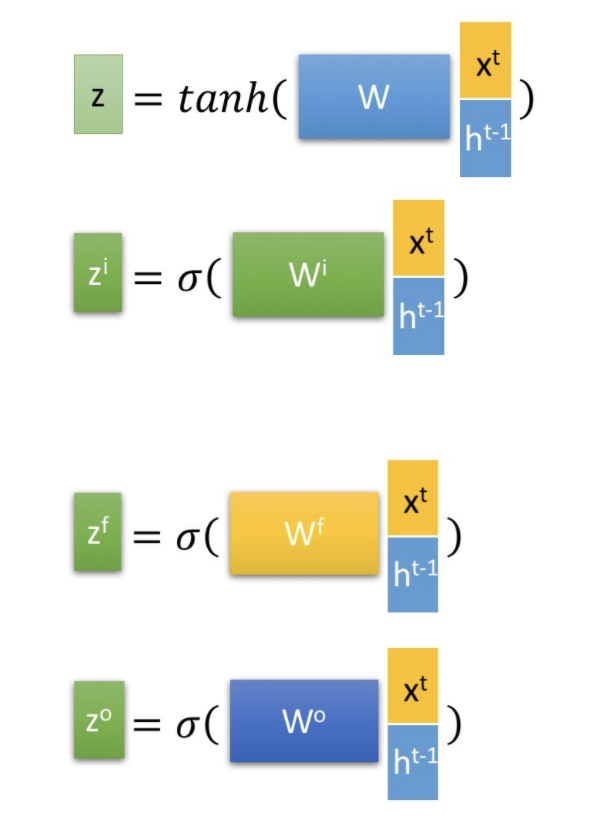
\includegraphics[width=.4\textwidth]{fig/LSTM_Four_States.png}
\end{figure}

其中,$z^f, z^i, z^o$是由拼接向量乘以权重矩阵之后,再通过一个 sigmoid  激活函数转换成0到1之间的数值,来作为一种门控状态。而 $z$ 则是将结果通过一个 tanh 激活函数将转换成-1到1之间的值(这里使用 tanh是因为这里是将其做为输入数据,而不是门控信号)。

下面开始进一步介绍这四个状态在LSTM内部的使用。、
\subsection{LSTM 的四个状态}
\begin{figure}[H]
    \centering
    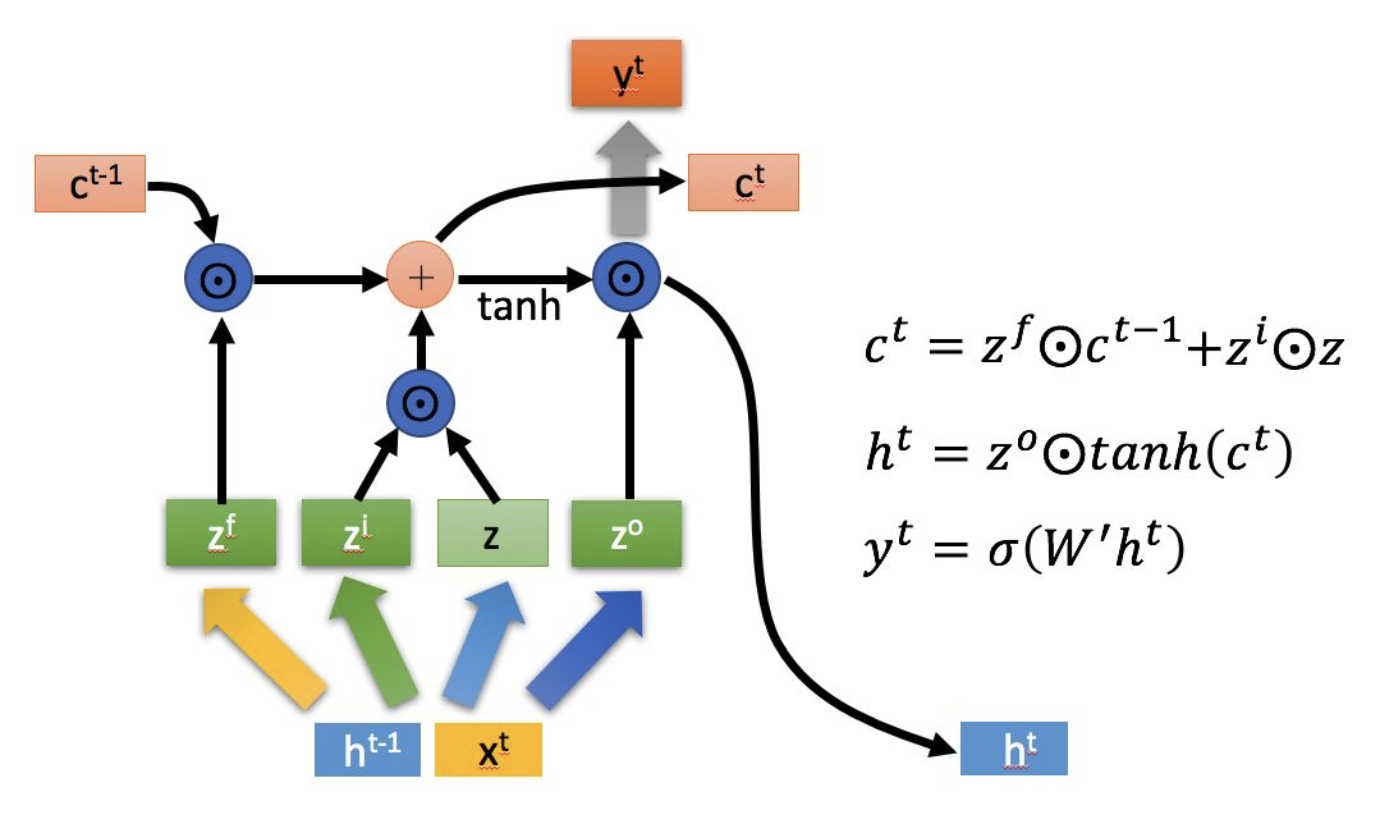
\includegraphics[width=.8\textwidth]{fig/LSTM_Four_States_Detail.png}
\end{figure}

$\odot$ 是Hadamard Product,也就是操作矩阵中对应的元素相乘,因此要求两个相乘矩阵是同型的。 $\oplus$ 则代表进行矩阵加法。

LSTM内部主要有三个阶段:

1. \textbf{忘记阶段}。这个阶段主要是对上一个节点传进来的输入进行选择性忘记。简单来说就是会 “忘记不重要的,记住重要的”。

具体来说是通过计算得到的$z^f$(f表示forget)来作为忘记门控,来控制上一个状态的 $c^{t-1}$ 哪些需要留哪些需要忘。

2. \textbf{选择记忆阶段}。这个阶段将这个阶段的输入有选择性地进行“记忆”。主要是会对输入 $x^t$ 进行选择记忆。哪些重要则着重记录下来,哪些不重要,则少记一些。当前的输入内容由前面计算得到的 $z$ 表示。而选择的门控信号则是由$z^i$ (i代表information)来进行控制。

将上面两步得到的结果相加,即可得到传输给下一个状态的$c^t$。也就是上图中的第一个公式。

3. \textbf{输出阶段}。这个阶段将决定哪些将会被当成当前状态的输出。主要是通过 $z^o$ 来进行控制的。并且还对上一阶段得到的 $c^o$进行了放缩(通过一个tanh激活函数进行变化)。

与普通RNN类似,输出$y^t$ 往往最终也是通过 $h^t$ 变化得到。

\subsection{LSTM 的门结构\cite{LSTM_Principle_And_Practice}}
在RNN里,$T_n$时刻的输入会把$T_{n-1}$的输出照单全收,而LSTM每个$T_n$时间点,存在两条线:主线剧情$c$和副线剧情$T_{n-1}$的输出,遗忘门等等都是副线剧情,他们通过权值影响主线剧情$c$,最后由$c$来决定$T_n$时刻的最终输出应该是多少。通过这种方式,我们可以避免离$T_n$比较近的时刻对于$T_n$的影响,同时也可以让我们的model记住之前比较久远但是对于此时刻的输出会很重要的信息。

\subsection{主线剧情$C_t$}
有了大概概念以后,我们就可以更加细致了解LSTM。我们先从剧情方面来讲,首先是主线剧情:
\begin{figure}[H]
    \centering
    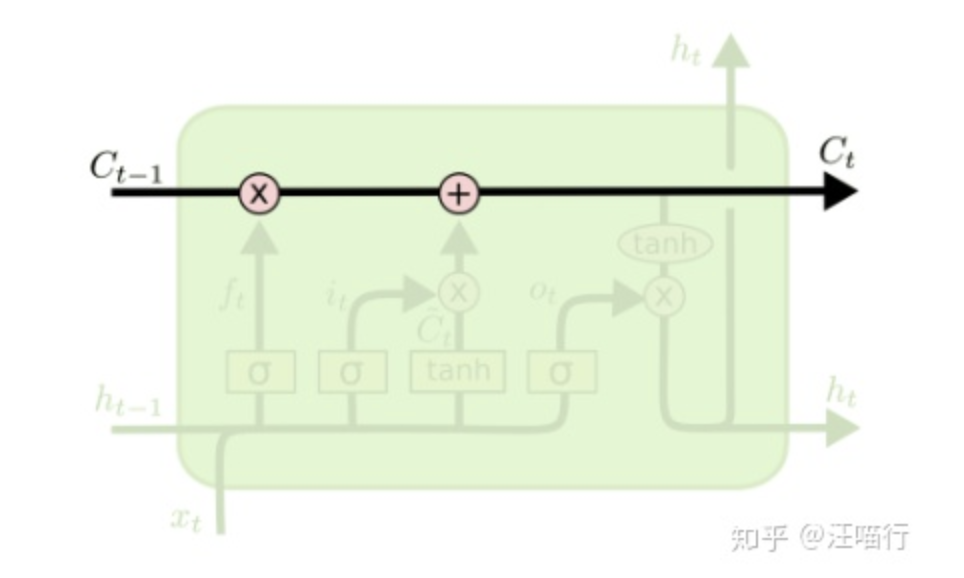
\includegraphics[width=.6\textwidth]{fig/LSTM_Main_Stream.png}
\end{figure}
在每个时间点$T_n$,都会有一个对应的状态$C_t$。这个$C_t$记录了之前的信息。在每个时间点,都可以通过调节权重的输入,遗忘等方式去修正$C_t$的状态。所以它可以类比一个主线剧情,好像男女主的爱情故事主线,中间每个时间点的他们的爱情状态都是不同的,会受到这个时间点的发生的事件/上个时间点的结果/以前发生的很久远的印象深刻的事情各种因素的影响,但是这个核心要素$C_t$是会随着时间不停改变但是一直传播下去的(一般来说能拍成电视剧,男女主的爱情$C_t$虽然波波折折,是最后美好又稳定的状态$C_t$是不会大改变的)。

\subsubsection{副线剧情:三个门}
讲完了男女主爱情的主线剧情,下面讲讲什么会影响吧。对于Ct来说主要会被影响的方式是通过sigmoid的方式:
\begin{figure}[H]
    \centering
    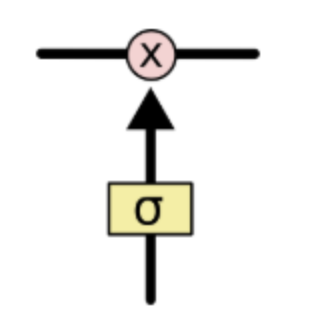
\includegraphics[width=.3\textwidth]{fig/LSTM_Gate_Sigmoid.png}
\end{figure}

通过sigmoid门来控制每个输入因素对于$C_t$的影响是多少,从全部不输入到全部输入都可以通过这个函数来做到。而会影响这个主线剧情的主要有三个门:遗忘门,输入门,输出门,下面一一介绍:

\textbf{遗忘门},和名字一样,表示上个时间点的状态我应该遗忘多少。对于$C_{t-1}$来说,会首先看上一个阶段的输出$h_{t-1}$和这个阶段的输入$x_{t}$,并通过sigmoid来确定要让$C_{t-1}$,来忘记多少,sigmoid=1表示要保存多一些$C_{t-1}$的比重,等于0表示完全忘记之前的$C_{t-1}$。
\begin{figure}[H]
    \centering
    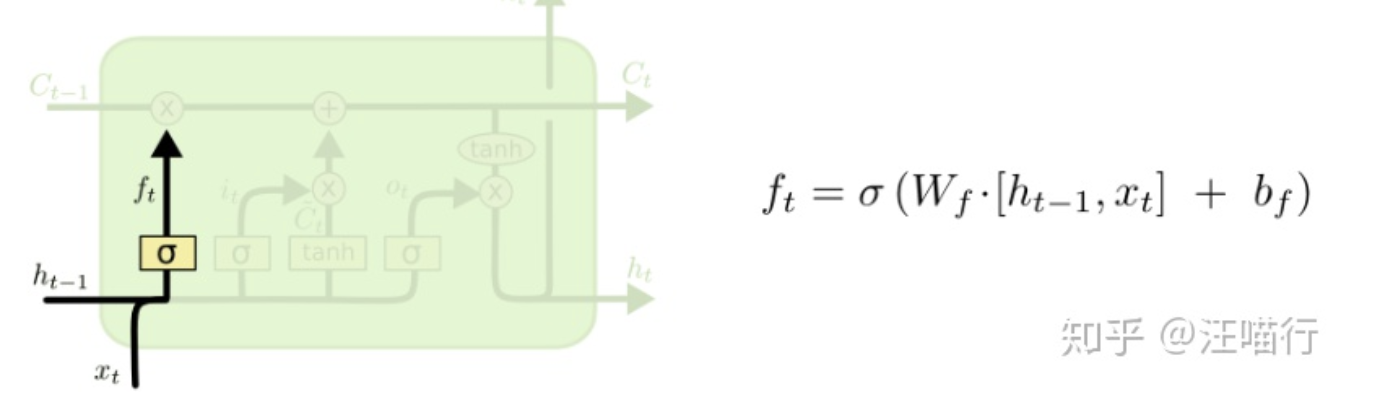
\includegraphics[width=.8\textwidth]{fig/LSTM_Gate_Forget.png}
\end{figure}

\textbf{输入门},首先会拿上一个阶段的输出$h_{t-1}$和这个阶段的输入$x_{t}$,通过sigmoid来控制现在要加多少进入主线剧情$C_t$,即第一个公式的含义;然后又会创建一个备选的$\tilde{C}t$,用tanh去控制要加入$C_t$的部分是多少。
\begin{figure}[H]
    \centering
    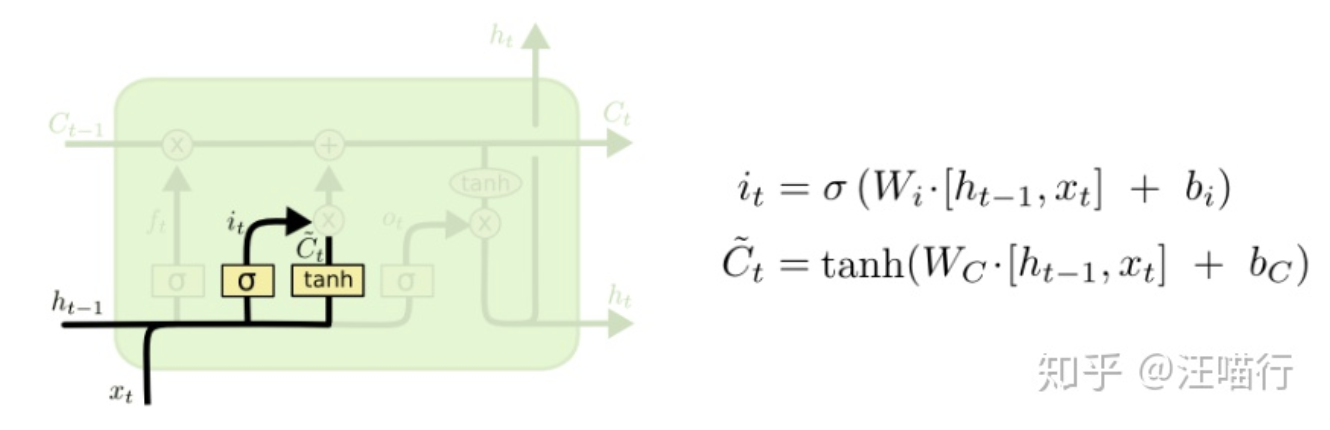
\includegraphics[width=.8\textwidth]{fig/LSTM_Gate_Input.png}
\end{figure}

之后通过把两个部分相乘,总共决定了要影响$C_t$的量是多少,加上之前的遗忘门的影响,可以写为:
\begin{figure}[H]
    \centering
    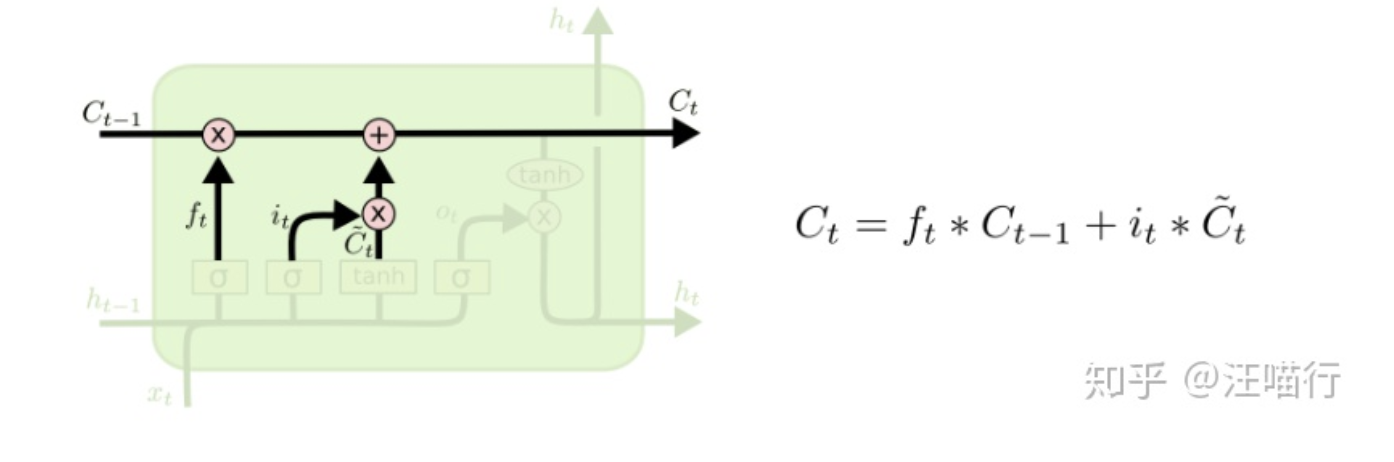
\includegraphics[width=.8\textwidth]{fig/LSTM_Gate_Forget_Input.png}
\end{figure}

\textbf{输出门},最后一步,有了对于 $C_t$的影响,我们最后看看到底想要输出多少:
\begin{figure}[H]
    \centering
    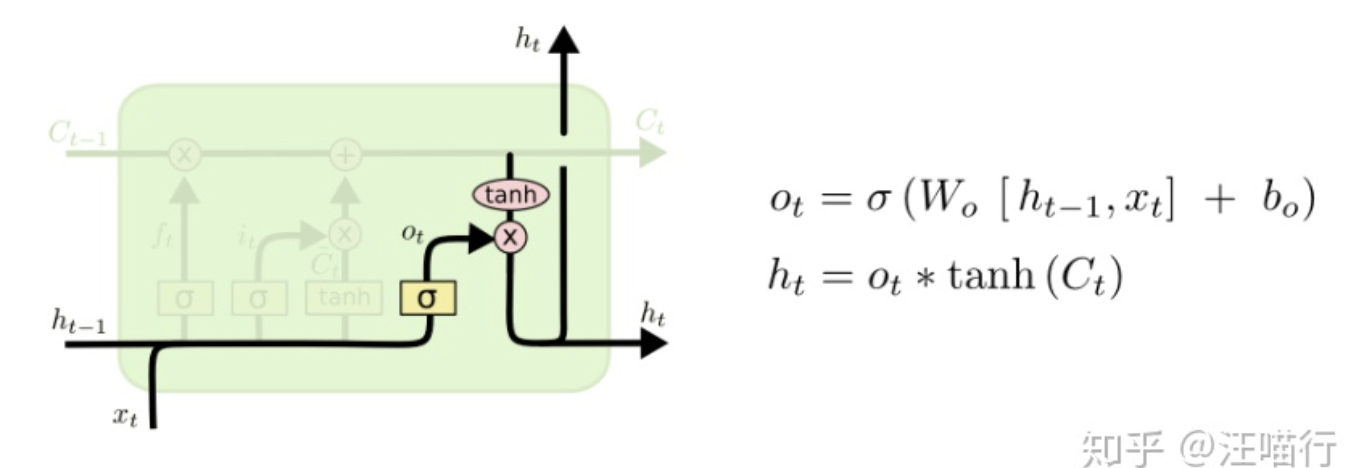
\includegraphics[width=.8\textwidth]{fig/LSTM_Gate_Output.png}
\end{figure}
首先我们通过sigmoid函数,来决定$C_t$的哪一部分需要被输出,即第一个公式的$o_t$;之后,我们把$C_t$放入tanh内,决定最后输出$C_t$的部分,并和$o_t$相乘,得到最后的输出。

\subsection{LSTM 总结}
以上,就是LSTM的内部结构。通过门控状态来控制传输状态,记住需要长时间记忆的,忘记不重要的信息;而不像普通的RNN那样只能够“呆萌”地仅有一种记忆叠加方式。对很多需要“长期记忆”的任务来说,尤其好用。

但也因为引入了很多内容,导致参数变多,也使得训练难度加大了很多。因此很多时候我们往往会使用效果和LSTM相当但参数更少的GRU来构建大训练量的模型。

\section{GRU\cite{Everyone_Can_Understand_GRU}}
\subsection{什么是GRU}
GRU(Gate Recurrent Unit)是循环神经网络(Recurrent Neural Network, RNN)的一种。和LSTM(Long-Short Term Memory)一样,也是为了解决长期记忆和反向传播中的梯度等问题而提出来的。

GRU和LSTM在很多情况下实际表现上相差无几,那么为什么我们要使用新人GRU(2014年提出)而不是相对经受了更多考验的LSTM(1997提出)呢。

简单来说,我们在我们的实验中选择GRU是因为它的实验效果与LSTM相似,但是更易于计算。相比LSTM,使用GRU能够达到相当的效果,并且相比之下更容易进行训练,能够很大程度上提高训练效率,因此很多时候会更倾向于使用GRU。

OK,那么为什么说GRU更容易进行训练呢,下面开始介绍一下GRU的内部结构。

\subsection{GRU浅析}
\subsubsection{GRU的输入输出结构}
GRU的输入输出结构与普通的RNN是一样的。

有一个当前的输入$x^t$,和上一个节点传递下来的隐状态(hidden state) $h^{t-1}$ ,这个隐状态包含了之前节点的相关信息。结合 $x^t$ 和 $h^{t-1}$,GRU会得到当前隐藏节点的输出 $y^t$ 和传递给下一个节点的隐状态 $h^t$。
\begin{figure}[H]
    \centering
    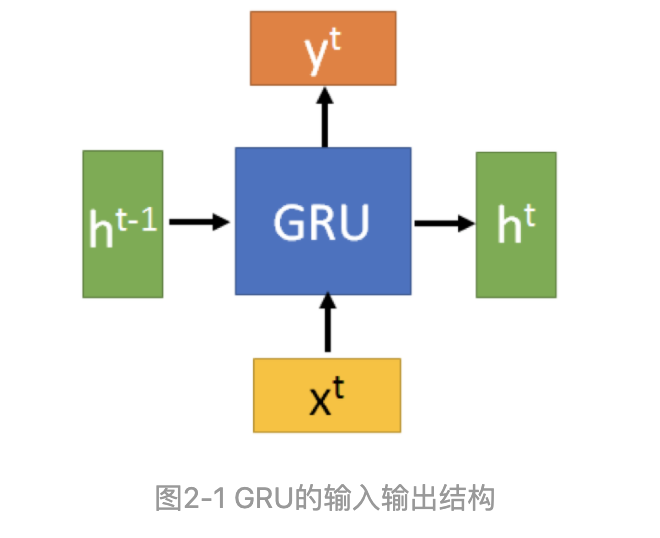
\includegraphics[width=.6\textwidth]{fig/GRU_Structure_InputOutput.png}
\end{figure}

\subsubsection{GRU的内部结构}
首先,我们先通过上一个传输下来的状态 $h^{t-1}$和当前节点的输入$x^t$来获取两个门控状态。如下图2-2所示,其中$r$控制重置的门控(reset gate),$z$ 为控制更新的门控(update gate)。
\begin{figure}[H]
    \centering
    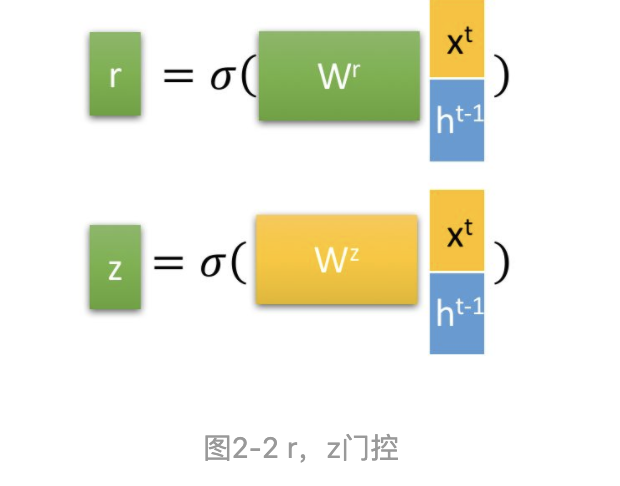
\includegraphics[width=.6\textwidth]{fig/GRU_RZ_Gate.png}
\end{figure}
 
得到门控信号之后,首先使用重置门控来得到“重置”之后的数据$h^{{t-1}'} = h^{t-1}\odot r$ ,再将 $h^{{t-1}'} $ 与输入$x^t$ 进行拼接,再通过一个tanh激活函数来将数据放缩到-1~1的范围内。即得到如下所示的 $h'$ 。
\begin{figure}[H]
    \centering
    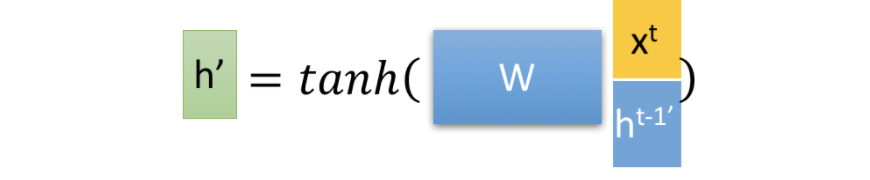
\includegraphics[width=.6\textwidth]{fig/GRU_h_pie.png}
\end{figure}

这里的$h'$ 主要是包含了当前输入的 $x^t$ 数据。有针对性地对$h'$添加到当前的隐藏状态,相当于”记忆了当前时刻的状态“。类似于LSTM的选择记忆阶段。
\begin{figure}[H]
    \centering
    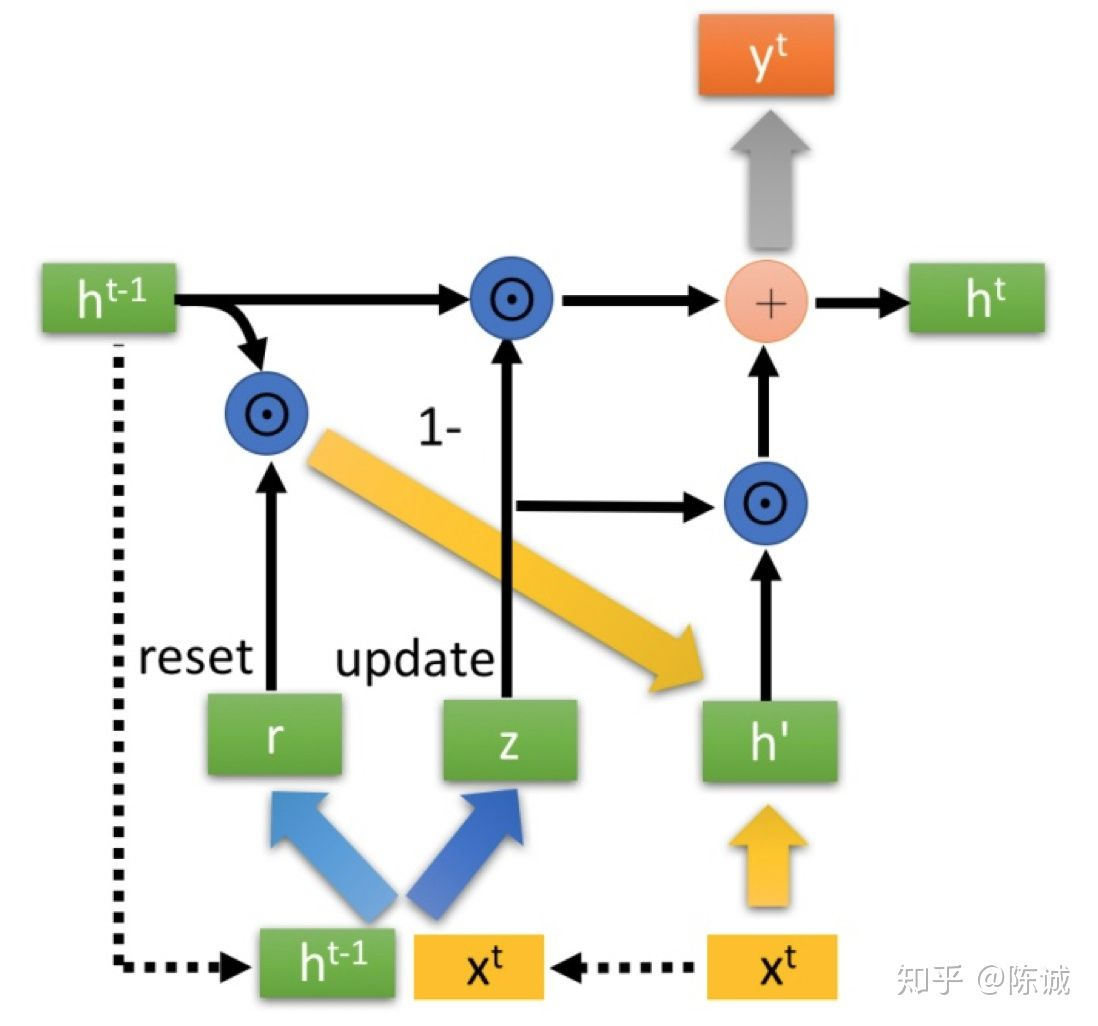
\includegraphics[width=.6\textwidth]{fig/GRU_Internal_Structure.jpg}
\end{figure}

最后介绍GRU最关键的一个步骤,我们可以称之为”更新记忆“阶段。

在这个阶段,我们同时进行了遗忘和记忆两个步骤。我们使用了先前得到的更新门控$z$(update gate),更新表示式如下:
$$
h^t = (1-z) \odot h^{t-1} + z \odot h'
$$

首先再次强调一下,门控信号(这里的$z$)的范围为0~1。门控信号越接近1,代表”记忆“下来的数据越多;而越接近0则代表”遗忘“的越多。

GRU很聪明的一点就在于,我们使用了同一个门控 $z$就同时可以进行遗忘和选择记忆(LSTM则要使用多个门控)。
\begin{itemize}
\setlength{\itemsep}{0pt}
\setlength{\parsep}{0pt}
\setlength{\parskip}{0pt}
    \item $ (1-z) \odot h^{t-1}$:表示对原本隐藏状态的选择性“遗忘”。这里的 $1-z$可以想象成遗忘门(forget gate),忘记$h^{t-1}$维度中一些不重要的信息;
    \item $z \odot h'$ : 表示对包含当前节点信息的 $h'$ 进行选择性”记忆“。与上面类似,这里的$1-z$同理会忘记$h'$  维度中的一些不重要的信息。或者,这里我们更应当看做是对$h'$  维度中的某些信息进行选择;
    \item $h^t = (1-z) \odot h^{t-1} + z \odot h'$ :结合上述,这一步的操作就是忘记传递下来的$h^{t-1}$ 中的某些维度信息,并加入当前节点输入的某些维度信息。
\end{itemize}


%\printbibliography
\bibliography{../ref}
\bibliographystyle{IEEEtran}
\end{document}